\documentclass{urdpl}     % praca w języku polskim

% Lista wszystkich języków stanowiących języki pozycji bibliograficznych użytych w pracy.
% (Zgodnie z zasadami tworzenia bibliografii każda pozycja powinna zostać utworzona zgodnie z zasadami języka, w którym dana publikacja została napisana.)
\usepackage[english,polish]{babel}

% Użyj polskiego łamania wyrazów (zamiast domyślnego angielskiego).
\usepackage{polski}

\usepackage[utf8]{inputenc}

% dodatkowe pakiety

\usepackage{mathtools}
\usepackage{amsfonts}
\usepackage{amsmath}
\usepackage{amsthm}
\usepackage[hidelinks]{hyperref}
\usepackage{float}
\usepackage{listings}
\usepackage{graphicx}
\usepackage{subcaption}
\usepackage{booktabs} % Dla \toprule, \midrule, \bottomrule
\usepackage{multirow} 
\usepackage{tabularx} 
\usepackage{amssymb} 
\usepackage{listings}
\usepackage{xcolor}
\usepackage{array}
\usepackage{makecell}
\usepackage[flushleft]{threeparttable}
\usepackage[normalem]{ulem}
\usepackage{lineno}
\usepackage{makecell} %
\usepackage{csquotes}
\usepackage{courier}

% ------------------------
% --- < listingi > ---

\usepackage{listings}
\lstloadlanguages{TeX}
\renewcommand{\lstlistlistingname}{Spis listingów}
\renewcommand{\lstlistingname}{Listing}

\lstset{
	literate={ą}{{\k{a}}}1
           {ć}{{\'c}}1
           {ę}{{\k{e}}}1
           {ó}{{\'o}}1
           {ń}{{\'n}}1
           {ł}{{\l{}}}1
           {ś}{{\'s}}1
           {ź}{{\'z}}1
           {ż}{{\.z}}1
           {Ą}{{\k{A}}}1
           {Ć}{{\'C}}1
           {Ę}{{\k{E}}}1
           {Ó}{{\'O}}1
           {Ń}{{\'N}}1
           {Ł}{{\L{}}}1
           {Ś}{{\'S}}1
           {Ź}{{\'Z}}1
           {Ż}{{\.Z}}1,
	basicstyle=\footnotesize\ttfamily,
}

% defninicja stylu python
\lstdefinestyle{stylePython}{
    language=Python,
    commentstyle=\color{green},          % Kolor komentarzy
    keywordstyle=\color{blue},           % Kolor słów kluczowych
    numberstyle=\tiny\color{gray},       % Kolor i styl numerów linii
    stringstyle=\color{red},             % Kolor ciągów znaków
    basicstyle=\ttfamily\footnotesize,   % Podstawowy styl kodu
    breakatwhitespace=false,             % Automatyczne dzielenie wierszy
    breaklines=true,                     % Dzielenie długich linii
    keepspaces=true,                     % Zachowanie spacji
    numbers=left,                        % Numery linii po lewej
    numbersep=5pt,                       % Odstęp numerów od kodu
    showspaces=false,                    % Nie pokazuj spacji
    showstringspaces=false,              % Nie pokazuj spacji w ciągach znaków
    showtabs=false,                      % Nie pokazuj tabulacji
    tabsize=2                            % Rozmiar tabulacji
}

% defnicja stylu JAVA
\lstdefinestyle{javaStyle}{
    language=Java,
    basicstyle=\ttfamily\footnotesize,
    keywordstyle=\color{blue},
    commentstyle=\color{green!50!black}\itshape,
    stringstyle=\color{green},
    numberstyle=\tiny\color{gray},
    numbers=left,
    numbersep=5pt,                       % Odstęp numerów od kodu
    stepnumber=1,
    showspaces=false,                    % Nie pokazuj spacji
    tabsize=2,
    showstringspaces=false,
    breaklines=true,
    breakatwhitespace=false,             % Automatyczne dzielenie wierszy
    showtabs=false,                      % Nie pokazuj tabulacji
    keepspaces=true                    % Zachowanie spacji
}

\definecolor{stringcolor}{RGB}{163,21,21}    % pomarańczowy - stringi
\definecolor{typecolor}{RGB}{43, 145, 176}     % ciemny fiolet - klasy, typy

\lstdefinestyle{csStyle}{
    language=[Sharp]C, % dla C#; można zmienić na Java
    basicstyle=\ttfamily\footnotesize,
    keywordstyle=\color{blue},
    stringstyle=\color{stringcolor},
    commentstyle=\color{green!50!black}\itshape,
    morekeywords={class, public, private, protected, static, void, string, int, new}, % dodatkowe słowa kluczowe
    emphstyle=\color{typecolor}\bfseries, % klasy na fioletowo
    numbers=left,
    numbersep=5pt,                       % Odstęp numerów od kodu
    numberstyle=\tiny\color{gray},
    stepnumber=1,
    breaklines=true,
    showspaces=false,                    % Nie pokazuj spacji
    tabsize=2,
    showstringspaces=false,
    breakatwhitespace=false,             % Automatyczne dzielenie wierszy
    showtabs=false,                      % Nie pokazuj tabulacji
    keepspaces=true                    % Zachowanie spacji  
}

\lstdefinestyle{matlabStyle}{
    language=Matlab,
    basicstyle=\ttfamily\footnotesize,  % Mała czcionka monospaced
    keywordstyle=\color{blue}\bfseries, % Słowa kluczowe na niebiesko i pogrubione
    stringstyle=\color{red},            % Ciągi znaków na czerwono
    commentstyle=\color{green!50!black}\itshape, % Komentarze na zielono, kursywa
    morekeywords={figure, imread, imshow, title, imhist, histeq, graythresh, imbinarize, stretchlim, imadjust}, % Dodatkowe słowa kluczowe MATLAB
    numbers=left,                        % Numeracja linii po lewej
    numbersep=5pt,                       % Odstęp numerów od kodu
    numberstyle=\tiny\color{gray},       % Mała, szara czcionka numerów linii
    stepnumber=1,                         % Numeracja co 1 linię
    breaklines=true,                      % Łamanie długich linii
    showspaces=false,                     % Nie pokazuj spacji
    showstringspaces=false,               % Nie pokazuj spacji w stringach
    showtabs=false,                        % Nie pokazuj tabulatorów
    tabsize=4,                             % Tabulacja 4 spacje
    breakatwhitespace=false,               % Automatyczne łamanie wierszy
    keepspaces=true                        % Zachowanie spacji  
}

\definecolor{lightgray}{rgb}{0.9,0.9,0.9}
    % \definecolor{blue}{rgb}{0,0,1}
    \definecolor{green}{rgb}{0,0.6,0}
    % \definecolor{red}{rgb}{0.6,0,0}
    \definecolor{gray}{rgb}{0.5,0.5,0.5}

% % ------------------------
\AtBeginDocument{
	\renewcommand{\tablename}{Tabela}
	\renewcommand{\figurename}{Rys.}   
    \newcommand{\listingname}{Listing}
}

% ------------------------
% --- < tabele > ---

% defines the X column to use m (\parbox[c]) instead of p (`parbox[t]`)
\newcolumntype{C}[1]{>{\hsize=#1\hsize\centering\arraybackslash}X}


%---------------------------------------------------------------------------

\author{Oleksii Nawrocki}
\shortauthor{O. Nawrocki}
\noAlbum{oa131400}

\titlePL{Sprawozdanie z ćwiczeń laboratoryjnych z przedmiotu Biometryczne Systemy Zabezpieczeń}
\titleEN{Thesis in \LaTeX}

\shorttitlePL{Laboratorium z Biometrycznych Systemów Zabezpieczeń} % skrócona wersja tytułu jeśli jest bardzo długi
\shorttitleEN{Preparation of a long and fascinating thesis in \LaTeX}

\thesistype{Sprawozdania\\ Grupa: 02 \\Zespół nr: XX }

\thesisDone{Prowadzący}
\supervisor{dr Zbigniew Gomółka}
%\supervisor{Jan Nowak PhD}

\degreeprogramme{Informatyka}
%\degreeprogramme{Computer Science}

\date{2025}

\department{Instytut Informatyki}
%\department{Institute of Computer Science}

\faculty{Wydział Nauk Ścisłych i Technicznych}
%\faculty{Faculty of Science and Technology}



\setlength{\cftsecnumwidth}{10mm}

%---------------------------------------------------------------------------
\setcounter{secnumdepth}{4}
\brokenpenalty=10000\relax

% --------------------------------------------------------------------------
% główna część pracy
% --------------------------------------------------------------------------

\begin{document}

\titlepages

\tableofcontents

% dodanie poszczególnych rozdziałów 
\chapter{Laboratorium 1}
\label{cha:Lab001}
\makeatletter


% *********************************************************************
% w poniższej metryczce należy uzupełnić informacje o:
% - temacie ćwiczenia
% - numer ćwiczenia
% - numer grupy laboratoryjnej
% - numer zespołu
% - datę wykonania ćwiczenia oraz oddania ćwiczenia.
% *********************************************************************

\begin{table}[H]
    \centering
    \renewcommand{\tabularxcolumn}[1]{m{#1}}  % Dostosowanie kolumny do zawartości
    \newcolumntype{C}{>{\centering\arraybackslash}X}
    \begin{tabularx}{\linewidth}{|C|C|}
        \hline
        \multicolumn{2}{|c|}{\makecell{\textbf{\Large{Biometryczne Systemy Zabezpieczeń}} \\ \textbf{Ćwiczenia Laboratoryjne}}} \\ \hline
        \multicolumn{1}{|l|}{Temat}                    &              WPROWADZENIE DO BIBLIOTEKI MATLAB IMAGE PROCESSING ORAZ HISTOGRAMOWE METODY SEGMENTACJI OBRAZÓW.             \\ \hline
        \multicolumn{1}{|l|}{Ćwiczenie nr:}                    &      01                   \\ \hline
        \multicolumn{1}{|l|}{Autorzy:}                         &   \@author                              \\ \hline
        \multicolumn{1}{|l|}{Grupa laboratoryjna}                       &       02               \\ \hline
        \multicolumn{1}{|l|}{Zespół nr. }                       &    XX                  \\ \hline
        \multicolumn{1}{|l|}{Data wykonana ćwiczenia}         &  23.04.2025     \\ \hline
        \multicolumn{1}{|l|}{Data oddania ćwiczenia  }         &   13.05.2025     \\ \hline
    \end{tabularx}
\end{table}


\section{Cel ćwiczenia}

Celem laboratorium jest zapoznanie się z podstawowymi funkcjami biblioteki Image Processing Toolbox w MATLAB-ie oraz zastosowanie metod segmentacji obrazów opartych na analizie histogramu. Należy zapoznać się z materiałami i przykładami zawartymi w niniejszych materiałach oraz zaproponować rozwiązania dla zadań do samodzielnego rozwiązania. Rozwiązania należy umieścić w sprawozdaniu, zgodnie z wymaganiami.

\section{Wstęp teoretyczny}
Histogram obrazu to funkcja przedstawiająca rozkład wartości pikseli w obrazie. Może być wykorzystywany do:
\begin{itemize}
	\item Poprawy kontrastu obrazu (rozciąganie histogramu, wyrównywanie histogramu),
	\item Segmentacji obrazu na podstawie progów jasności (np. metoda Otsu),
	\item Analizy jakości obrazu, w tym identyfikacji prześwietlonych lub niedoświetlonych obszarów.
\end{itemize}

Histogram w obrazie monochromatycznym można obliczyć za pomocą funkcji $h(k)$, określającej liczbę pikseli o poziomie jasności $k$:
\begin{equation}
	h(k) = \sum_{(x,y) \in \Omega} \delta(I(x,y) - k),
\end{equation}
gdzie $\delta$ to funkcja Kroneckera, a $\Omega$ oznacza zbiór pikseli w obrazie.

\section{Opis wykorzystywanego oprogramowania i narzędzi}
Do przeprowadzenia eksperymentu wykorzystano środowisko MATLAB oraz bibliotekę Image Processing Toolbox. Kluczowe funkcje wykorzystane w analizie to:
\begin{itemize}
	\item \texttt{imhist} - obliczanie histogramu obrazu,
	\item \texttt{imadjust} - rozciąganie histogramu,
	\item \texttt{histeq} - wyrównywanie histogramu,
	\item \texttt{graythresh} oraz \texttt{imbinarize} - segmentacja metodą Otsu.
\end{itemize}

\section{Zadania do wykonania samodzielnego}

\subsection{Zadanie 1}

\subsubsection{Treść}
\textbf{Konwersja obrazu na różne formaty przy użyciu MATLAB i Image Processing Toolbox:}

Użyj funkcji dostępnych w bibliotece IPT w MATLAB-ie do przekształcenia obrazu. Na Rys. 9
przedstawiono schemat przepływu i konwersji różnych typów obrazów w MATLAB-ie,
z wykorzystaniem funkcji dostępnych w IPT.

\subsubsection{Pytania do analizy}

\begin{itemize}
	\item Jak zmienia się zakres wartości pikseli w kolejnych przekształceniach?
	
	\begin{itemize}
		\item RGB: 3 kanały (R, G, B), każdy z zakresem [0, 255]
		\item Monochromatyczny (gray): pojedynczy kanał, zakres [0, 255]
		\item Binarny: dwa poziomy – 0 (czarny) i 1 (biały)
		\item Indeksowany: każdy piksel to indeks w tablicy kolorów (zazwyczaj 0–255 przy 256 kolorach)
	\end{itemize}

	\item Jaka jest różnica w zajmowanej pamięci między różnymi formatami obrazów?

	\begin{itemize}
		\item \textbf{RGB}: największy rozmiar – 3 bajty na piksel (8 bitów × 3 kanały).
		\item \textbf{Gray}: 1 bajt na piksel.
		\item \textbf{Binarny}: 1 bit na piksel (oszczędność miejsca).
		\item \textbf{Indeksowany}: 1 bajt na piksel + osobna tablica kolorów (colormap).
	\end{itemize}

	\item Jakie mogą być zastosowania obrazów indeksowanych i binarnych w praktyce?

	\begin{itemize}
		\item Indeksowane:
		
		\begin{itemize}
			\item kompresja obrazów do GIF.
			\item aplikacje z ograniczoną paletą barw (np. grafika retro, przeglądarki).
		\end{itemize}
		
		\item Binarne:
		
		\begin{itemize}
			\item analiza obiektów (segmentacja, maski).
			\item OCR (rozpoznawanie tekstu).
			\item wykrywanie krawędzi, konturów.
		\end{itemize}
	\end{itemize}

\end{itemize}

\subsubsection{Przykładowy program}
\lstinputlisting[style= matlabStyle, caption= Wczytanie obrazu i stworzenie konwersji, label=Lab001_l1]{src/Lab001/zadanie1.m}

\subsubsection{Obrazy}
\begin{figure}[H]
	\centering
	\begin{subfigure}[t]{0.45\linewidth}
		\centering
		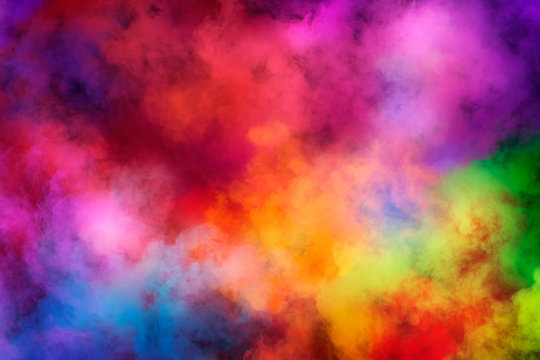
\includegraphics[width=\linewidth]{src/Lab001/zadanie1images/obraz_rgb.png}
		\caption{Obraz RGB}
		\label{fig:rgb}
	\end{subfigure}
	\hfill
	\begin{subfigure}[t]{0.45\linewidth}
		\centering
		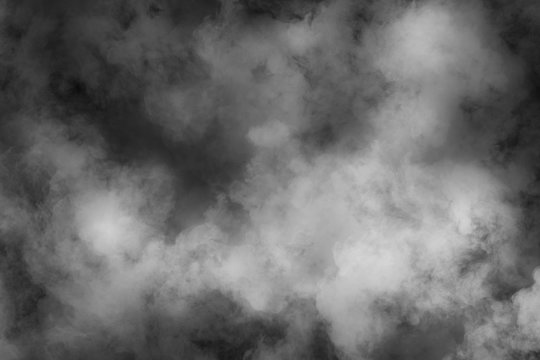
\includegraphics[width=\linewidth]{src/Lab001/zadanie1images/obraz_szary.png}
		\caption{Obraz szary}
		\label{fig:gray}
	\end{subfigure}
	
	\begin{subfigure}[t]{0.45\linewidth}
		\centering
		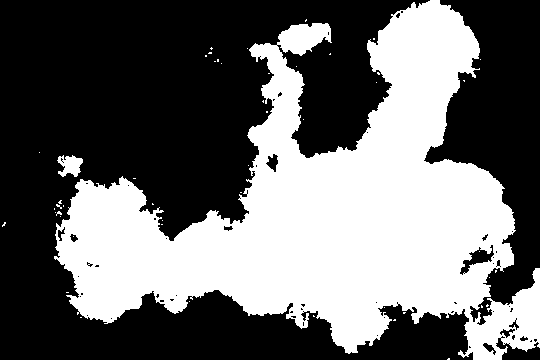
\includegraphics[width=\linewidth]{src/Lab001/zadanie1images/obraz_binarny.png}
		\caption{Obraz binarny}
		\label{fig:binary}
	\end{subfigure}
	\hfill
	\begin{subfigure}[t]{0.45\linewidth}
		\centering
		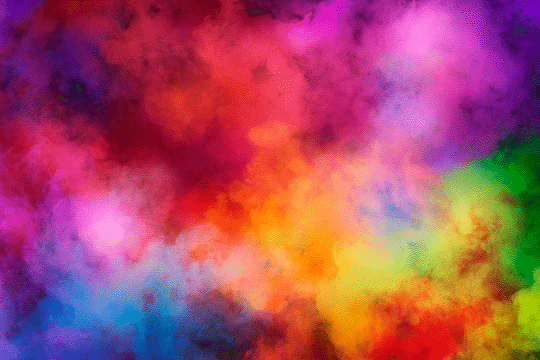
\includegraphics[width=\linewidth]{src/Lab001/zadanie1images/obraz_indeksowany.png}
		\caption{Obraz indeksowany}
		\label{fig:indexed}
	\end{subfigure}
	
	\begin{subfigure}[t]{0.45\linewidth}
		\centering
		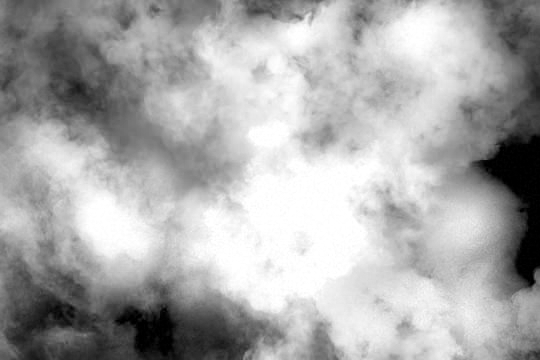
\includegraphics[width=\linewidth]{src/Lab001/zadanie1images/kanal_czerwony.png}
		\caption{Kanał czerwony}
		\label{fig:red}
	\end{subfigure}
	\hfill
	\begin{subfigure}[t]{0.45\linewidth}
		\centering
		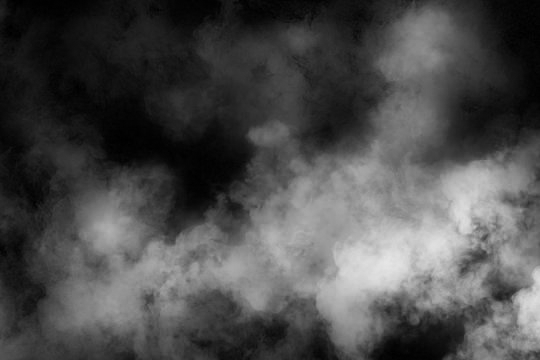
\includegraphics[width=\linewidth]{src/Lab001/zadanie1images/kanal_zielony.png}
		\caption{Kanał zielony}
		\label{fig:green}
	\end{subfigure}
	
	\begin{subfigure}[t]{0.45\linewidth}
		\centering
		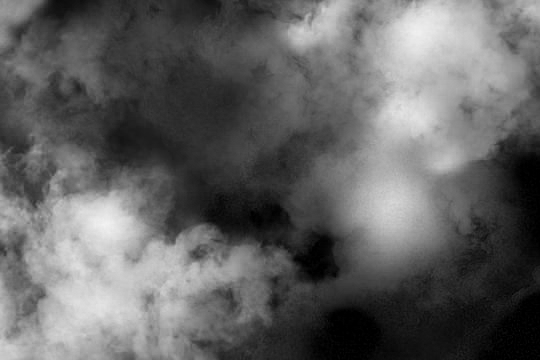
\includegraphics[width=\linewidth]{src/Lab001/zadanie1images/kanal_niebieski.png}
		\caption{Kanał niebieski}
		\label{fig:blue}
	\end{subfigure}
	
	\caption{Wizualizacja obrazów w różnych formatach i kanałach.}
	\label{fig:all_images1}
\end{figure}

\clearpage

\subsection{Zadanie 2}

\subsubsection{Treść}

\textbf{Zadanie 2. Histogram i operacje na histogramie.}

W Matlab zaproponuj program, który pozwoli na:

\begin{itemize}
	\item Wczytanie obrazu w skali szarości (imread → rgb2gray jeśli potrzeba).
	\item Obliczenie i wyświetlenie histogramu obrazu (imhist).
	\item Wykonaj rozciąganie histogramu (imadjust + stretchlim) i porównaj obraz przed i po operacji.
	\item Wykonaj wyrównanie histogramu (histeq) i porównaj wynik z oryginalnym obrazem oraz z histogramem rozciągniętym.
	\item Wyświetl histogramy wszystkich przekształconych obrazów.
\end{itemize}

\subsubsection{Przykładowy program}
\lstinputlisting[style= matlabStyle, caption= Wczytanie obrazu i przetwarzanie obrazu histogramami, label=Lab001_l2]{src/Lab001/zadanie2.m}
\clearpage

\subsubsection{Obrazy}

\begin{figure}[H]
	\begin{subfigure}[t]{0.45\linewidth}
		\centering
		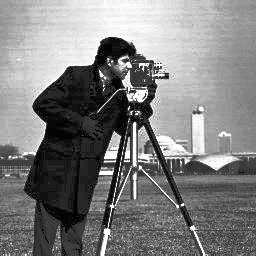
\includegraphics[width=\linewidth]{src/Lab001/zadanie2images/obraz_equalized.png}
		\caption{Obraz wyrównany}
		\label{fig:equ}
	\end{subfigure}
	\hfill
	\begin{subfigure}[t]{0.45\linewidth}
		\centering
		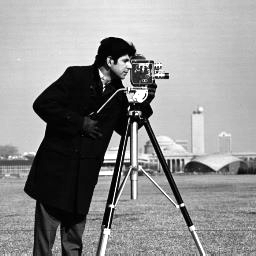
\includegraphics[width=\linewidth]{src/Lab001/zadanie2images/obraz_stretched.png}
		\caption{Obraz rozciągnięty}
		\label{fig:stretched}
	\end{subfigure}
		
	\caption{Wizualizacja rozciągania i wyrównywania obrazów}
	\label{fig:all_images2} 
\end{figure}

\subsubsection{Pytania do analizy}

\begin{itemize}
	\item Jaka jest różnica między rozciąganiem a wyrównywaniem histogramu?
	
	\begin{itemize}
		\item Rozciąganie (stretching): zmienia zakres jasności, przekształcając piksele tak, by rozciągnąć istniejący histogram do pełnego zakresu (np. 0–255).
		\item Wyrównywanie (equalization): zmienia rozkład jasności, aby histogram był możliwie równomierny – poprawiając kontrast globalnie.
	\end{itemize}
	
	\item Która metoda daje lepsze wyniki poprawy kontrastu?
	
	\begin{itemize}
		\item Dla obrazów o niskim kontraście — wyrównanie często działa lepiej.
		\item Dla obrazów z dobrze rozłożonymi poziomami jasności — rozciąganie może być wystarczające i mniej inwazyjne.
	\end{itemize}
	
	\item Jakie są potencjalne zastosowania tych technik?
	\begin{itemize}
		\item Poprawa jakości obrazów w:
		\begin{itemize}
			\item medycynie (np. obrazowanie rentgenowskie),
			\item nadzorze wizyjnym (monitoring),
			\item przetwarzaniu zdjęć satelitarnych,
			\item OCR (rozpoznawanie tekstu),	
			\item automatycznej analizy obrazów przemysłowych.
		\end{itemize}
	\end{itemize}
\end{itemize}

\clearpage

\subsection{Zadanie 3}

\subsubsection{Treść}
\textbf{Zadanie 3. Segmentacja obrazu na podstawie histogramu.}

W Matlab zaproponuj program, który pozwoli na:

\begin{itemize}
	\item Wczytanie obrazu w skali szarości.
	\item Obliczenie histogramu obrazu (imhist) i znalezienie potencjalnego progu segmentacji.
	\item Przeprowadź ręczną segmentację obrazu, stosując różne wartości progowe (BW = I > threshold).
	\item Zastosuj automatyczną segmentację metodą Otsu (graythresh + imbinarize).
	\item Porównaj efekty różnych progowań, wyświetlając wyniki obok siebie.
\end{itemize}

\subsubsection{Przykładowy program}

\lstinputlisting[style= matlabStyle, caption= Wczytanie obrazu i segmentacja na podstawie histogramu, label=Lab001_l3]{src/Lab001/zadanie3.m}
\clearpage

\subsubsection{Obrazy}

\begin{figure}[H]
	\begin{subfigure}[t]{0.45\linewidth}
		\centering
		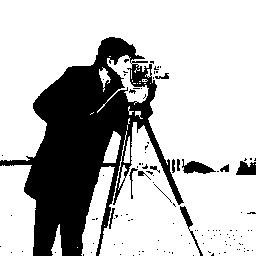
\includegraphics[width=\linewidth]{src/Lab001/zadanie3images/progowanie_80.png}
		\caption{Progowanie 80}
		\label{fig:prog80}
	\end{subfigure}
	\hfill
	\begin{subfigure}[t]{0.45\linewidth}
		\centering
		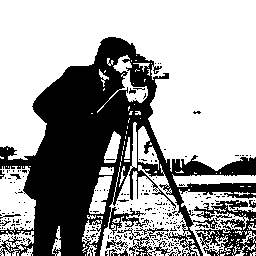
\includegraphics[width=\linewidth]{src/Lab001/zadanie3images/progowanie_120.png}
		\caption{Progowanie 120}
		\label{fig:prog120}
	\end{subfigure}
	
	\begin{subfigure}[t]{0.45\linewidth}
		\centering
		
\includegraphics[width=\linewidth]{src/Lab001/zadanie3images/progowanie_160.png}
		\caption{Progowanie 160}
		\label{fig:prog160}
	\end{subfigure}
	\hfill
	\begin{subfigure}[t]{0.45\linewidth}
		\centering
		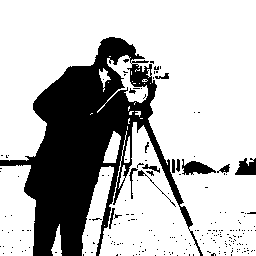
\includegraphics[width=\linewidth]{src/Lab001/zadanie3images/segmentacja_otsu.png}
		\caption{Segmentacja Otsu}
		\label{fig:sem_otsu}
	\end{subfigure}
	
	\caption{Operacje segmentowanie progowaniem oraz otsu.}
	\label{fig:all_images3} 
\end{figure}

\subsubsection{Pytania do analizy}

\begin{itemize}
	\item Jak dobrać optymalny próg segmentacji dla różnych obrazów?
	\begin{itemize}
		\item \textbf{Ręcznie}: na podstawie histogramu – szukamy wyraźnych "dolinek" (oddzielenie klas).
		\item \textbf{Automatycznie}: np. metoda Otsu – optymalizuje podział na dwie klasy o minimalnej wariancji wewnątrzklasowej.
	\end{itemize}
	
	\item Kiedy metoda Otsu jest skuteczniejsza niż segmentacja ręczna?
	\begin{itemize}
		\item Gdy histogram jest \textbf{dwumodalny} (dwa główne zbiory pikseli – tło i obiekt).
		\item Gdy chcemy \textbf{zautomatyzować} segmentację wielu obrazów bez ręcznego ustawiania progów.
		\item Gdy nie mamy wiedzy o zawartości obrazu i chcemy uzyskać ogólnie dobrą separację.
	\end{itemize}
	\clearpage
	
	\item Jakie mogą być praktyczne zastosowania binaryzacji?
	\begin{itemize}
		\item Detekcja i zliczanie obiektów (np. komórek w mikroskopii).
		\item OCR (rozpoznawanie tekstu).
		\item Analiza konturów i kształtów.
		\item Przemysł: detekcja defektów, systemy wizyjne.
		\item Monitoring: wykrywanie ruchu, segmentacja obiektów.
	\end{itemize}
\end{itemize}

\subsection{Zadanie 4}

\subsubsection{Treść}

\textbf{Zadania 4: Detekcja obiektów na obrazie binarnym.}

W Matlab zaproponuj program, który pozwoli na:

\begin{itemize}
	\item Wykonasz segmentację obrazu metodą Otsu i uzyskaj obraz binarny.
	\item Zidentyfikuj obiekty na obrazie binarnym za pomocą funkcji bwlabel lub regionprops.
	\item Wyznacz podstawowe właściwości wykrytych obiektów (np. powierzchnię, obwód).
	\item Narysuj prostokątne obramowania wokół wykrytych obiektów (rectangle).
	\item Zwizualizuj oryginalny obraz z nałożonymi obramowaniami.
\end{itemize}

\subsubsection{Przykładowy program}

\lstinputlisting[style= matlabStyle, caption= Wczytanie obrazu i dokonanie detekcji obiektów na obrazie, label=Lab001_l4]{src/Lab001/zadanie4.m}

\subsubsection{Obrazy}

\begin{figure}[H]
	\centering
	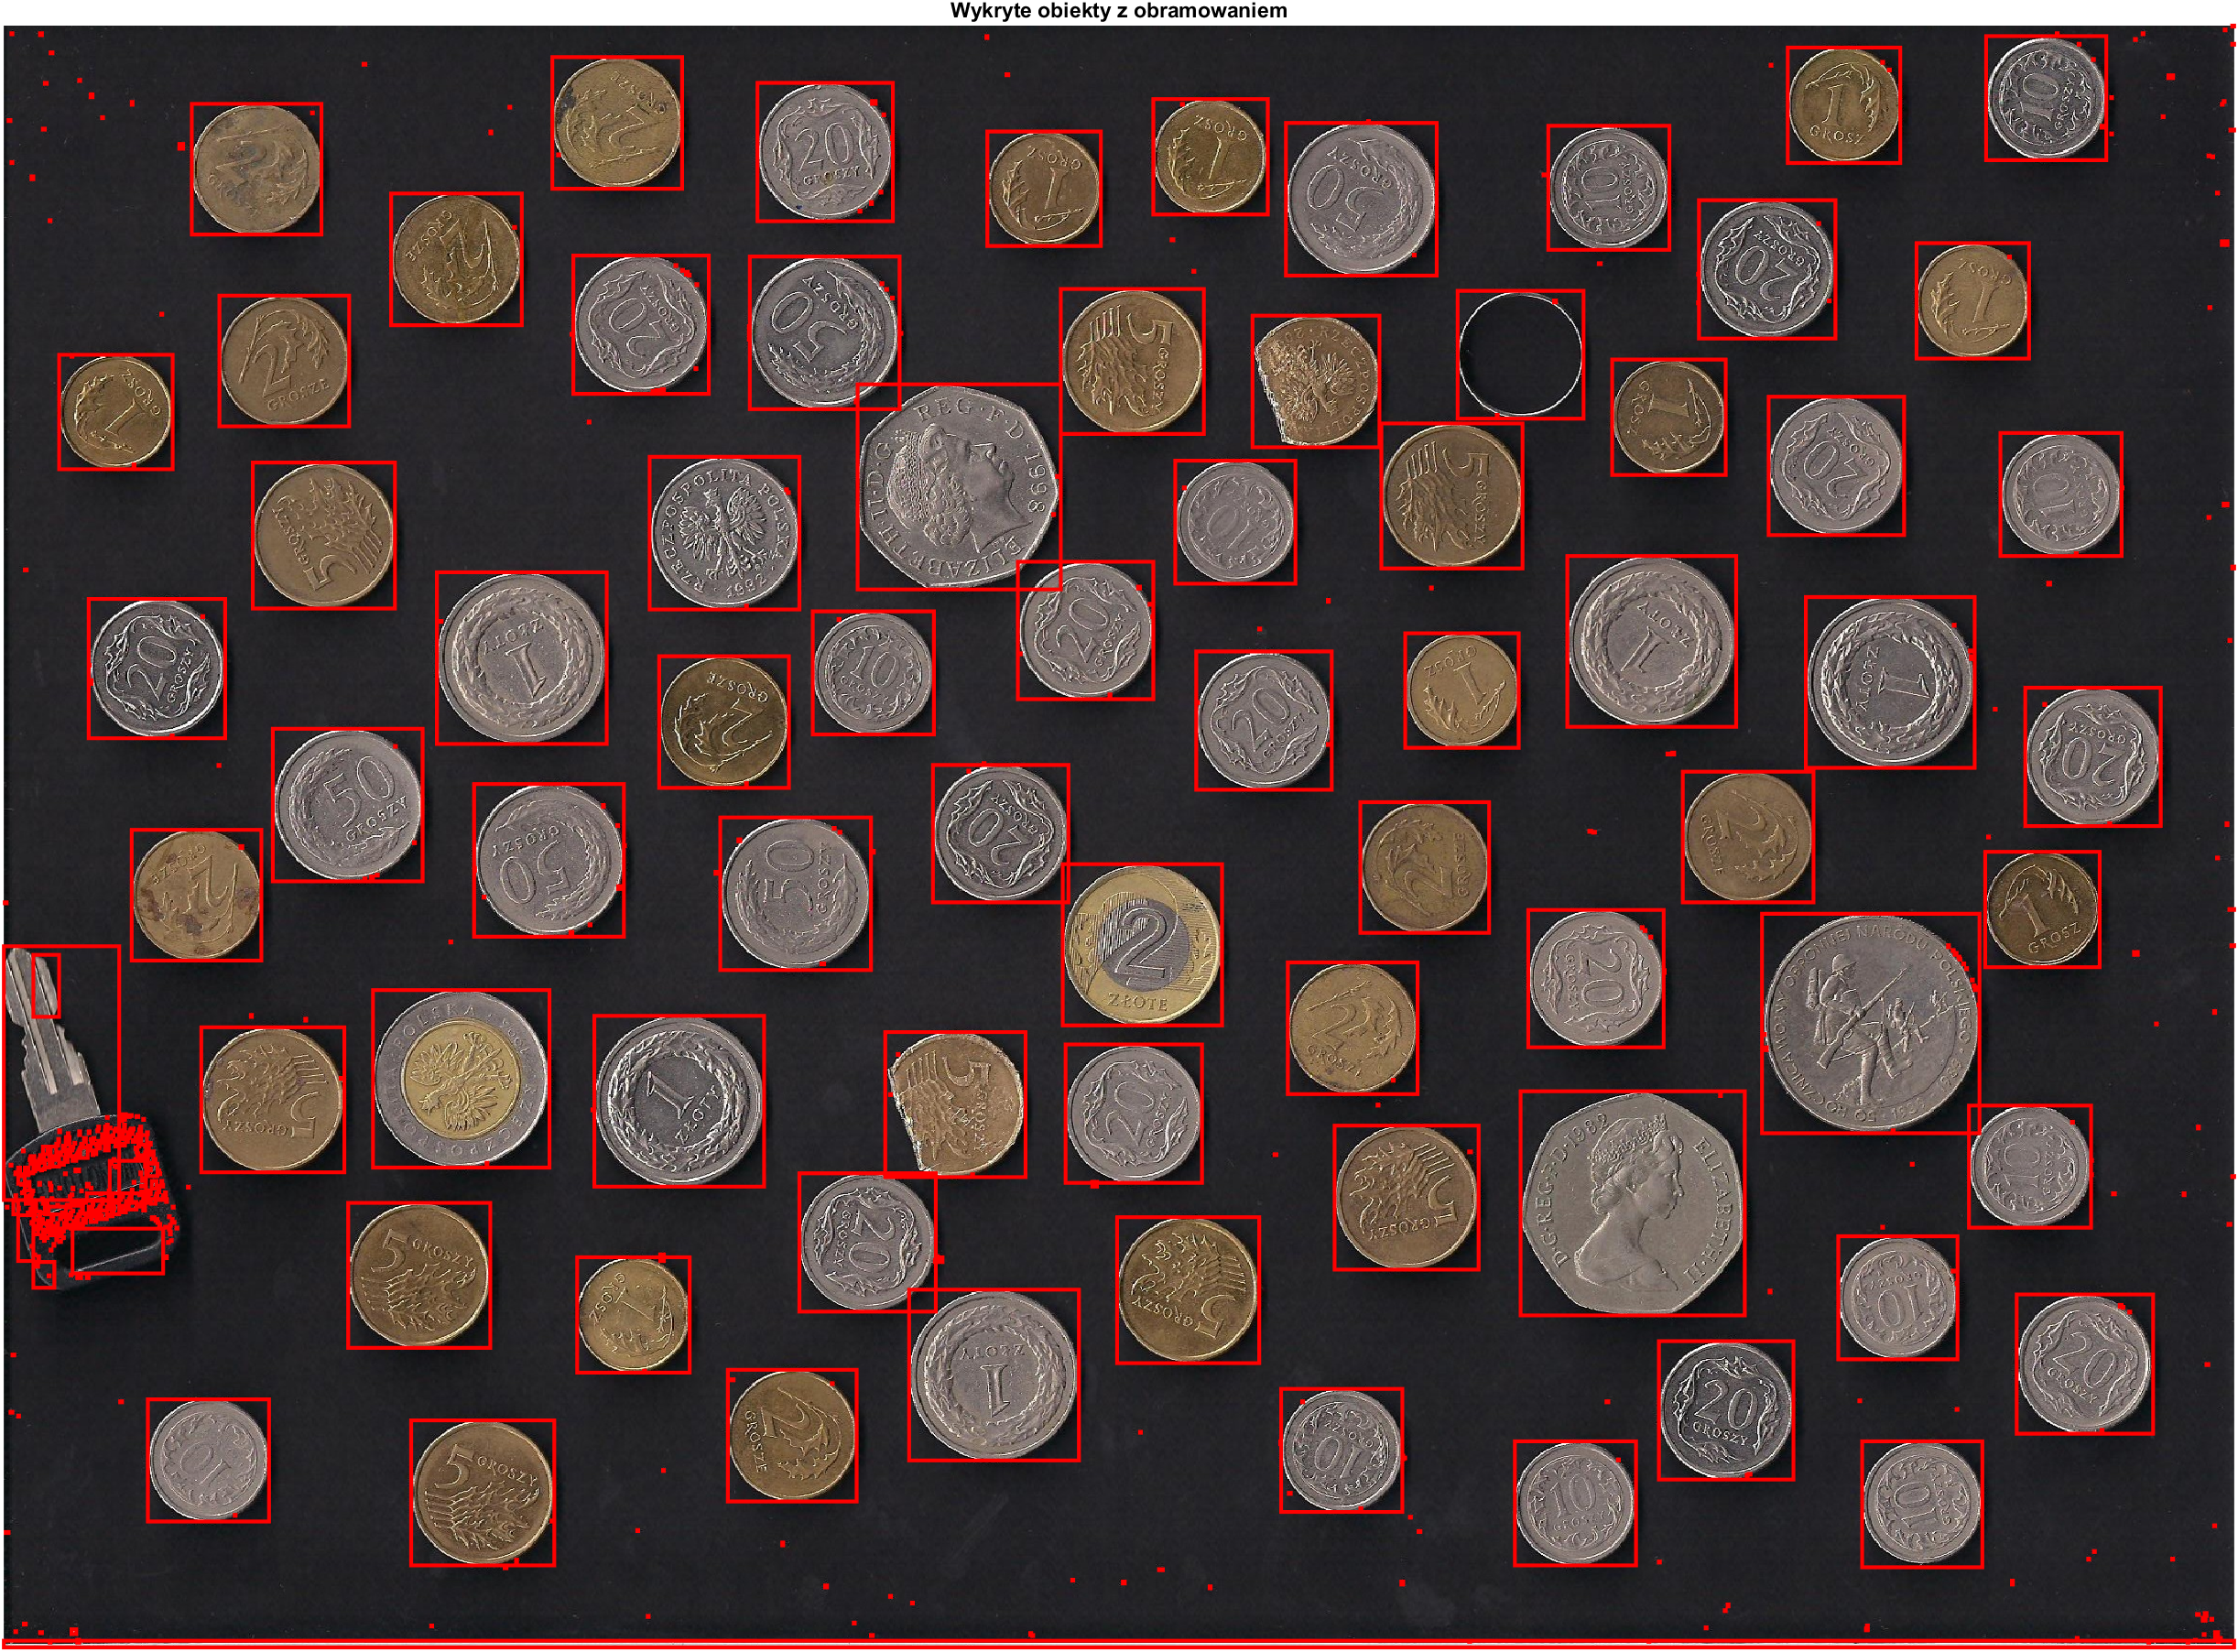
\includegraphics[width=0.7\linewidth]{src/Lab001/zadanie4images/obiekty_z_obramowaniem.png}\\
	\caption{Detekcja obiektów na obrazie.\label{fig:all_images4}}
\end{figure}

\subsubsection{Pytania do analizy}

\begin{enumerate}
	\item Jakie problemy mogą wystąpić przy detekcji obiektów w zależności od jakości segmentacji?
	\begin{itemize}
		\item Zbyt niska jakość segmentacji może prowadzić do:
		\begin{itemize}
			\item scalania sąsiadujących obiektów w jeden,
			\item pocięcia jednego obiektu na kilka części,
			\item pomijania obiektów o słabym kontraście,
			\item szumu – detekcji fałszywych obiektów.
		\end{itemize}
	\end{itemize}
	
	\item Jak można poprawić dokładność detekcji?
	\begin{itemize}
		\item Filtracja obrazu przed segmentacją (np. medfilt2, imgaussfilt).
		\item Morfologia: imopen, imclose, bwareaopen – usuwa drobne obiekty/szumy.
		\item Dostosowanie progu segmentacji ręcznie lub przez adaptacyjną binaryzację (adaptthresh).
		\item Użycie maski ROI lub filtrowanie po właściwościach (Area, Eccentricity, itp.).
	\end{itemize}
	
	\item Jakie są praktyczne zastosowania tej metody?
	\begin{itemize}
		\item \textbf{Biomedycyna}: zliczanie komórek, wykrywanie struktur w mikroskopii.
		\item \textbf{Przemysł}: kontrola jakości (np. wykrywanie wad, pomiar kształtu).
		\item \textbf{Robotyka/Widzenie maszynowe}: identyfikacja i lokalizacja obiektów.
		\item \textbf{Bezpieczeństwo}: wykrywanie tablic rejestracyjnych, ludzi, ruchu.
	\end{itemize}
\end{enumerate}

\subsection{Zadanie 5}

\subsubsection{Treść}

\textbf{Zadanie 5. Segmentacja wieloprogowa}

W Matlab zaproponuj program, który pozwoli na:

\begin{itemize}
	\item Wczytasz obraz w skali szarości.
	\item Obliczysz histogram obrazu i znajdźiesz dwa optymalne progi metodą Otsu (multithresh).
	\item Utwórz obraz segmentowany na trzy klasy (imquantize).
	\item Zwizualizuj wynik segmentacji z użyciem różnych kolorów (label2rgb).
	\item Porównaj segmentację wieloprogową z binaryzacją jednokryterialną.
\end{itemize}

\subsubsection{Przykładowy program}

\lstinputlisting[style= matlabStyle, caption= Wczytanie obrazu i dokonanie detekcji obiektów na obrazie, label=Lab001_l5]{src/Lab001/zadanie5.m}


\subsubsection{Obrazy}

\begin{figure}[H]
	\begin{subfigure}[t]{0.45\linewidth}
		\centering
		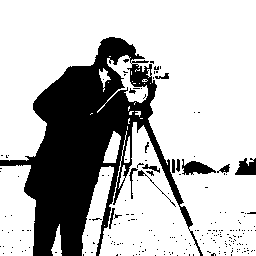
\includegraphics[width=\linewidth]{src/Lab001/zadanie5images/binaryzacja_otsu.png}
		\caption{Progowanie 80}
		\label{fig:bin_otsu}
	\end{subfigure}
	\hfill
	\begin{subfigure}[t]{0.45\linewidth}
		\centering
		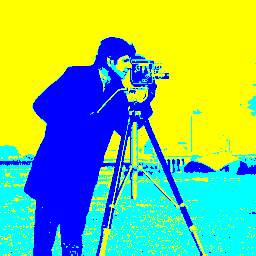
\includegraphics[width=\linewidth]{src/Lab001/zadanie5images/segmentacja_wieloprogowa.png}
		\caption{Progowanie 120}
		\label{fig:wiel_pr}
	\end{subfigure}
	
	\caption{Operacje segmentowanie wieloprogowego.}
	\label{fig:all_images5} 
\end{figure}

\subsubsection{Pytania do analizy}

\begin{enumerate}
	\item W jakich przypadkach segmentacja wieloprogowa daje lepsze wyniki niż binaryzacja?
	\begin{itemize}
		\item Gdy obraz zawiera \textbf{więcej niż dwa poziomy jasności} reprezentujące różne obiekty lub tło (np. tło, cień, obiekt).
		\item Przy obrazach z \textbf{wieloma klasami intensywności} – np. zdjęcia medyczne, zdjęcia z mikroskopu, obrazy satelitarne.
	\end{itemize}
	
	\item Jakie są ograniczenia segmentacji wieloprogowej?
	\begin{itemize}
		\item \textbf{Wymaga wiedzy} o liczbie klas (ile progów wyznaczyć).
		\item \textbf{Czasochłonna} przy większej liczbie progów lub dużych obrazach.
		\item Czasem nie sprawdza się przy słabym kontraście lub zaszumionym obrazie – klasy mogą się zlewać.
	\end{itemize}
	
	\item Jak można poprawić jakość segmentacji?
	\begin{itemize}
		\item \textbf{Filtracja} przed segmentacją (imgaussfilt, medfilt2).
		\item \textbf{Użycie morfologii} po segmentacji (imopen, imclose, bwareaopen).
		\item Dobór progów ręcznie lub przez adaptacyjne metody (adaptthresh).
		\item W połączeniu z analizą cech (regionprops) można odfiltrować obiekty niepasujące do oczekiwań.
	\end{itemize}
\end{enumerate}

\section{Wnioski}
Na podstawie przeprowadzonych eksperymentów można stwierdzić, że:
\begin{itemize}
    \item Histogram jest przydatnym narzędziem w analizie jakości obrazu biometrycznego.
    \item Wyrównanie histogramu poprawia kontrast i może zwiększać czytelność obrazu.
    \item Segmentacja oparta na histogramie, w szczególności metoda Otsu, pozwala na skuteczne wydzielenie istotnych cech obrazu.
\end{itemize}


\chapter{Laboratorium 2}
\label{cha:Lab002}
\makeatletter


% *********************************************************************
% w poniższej metryczce należy uzupełnić informacje o:
% - temacie ćwiczenia
% - numer ćwiczenia
% - numer grupy laboratoryjnej
% - numer zespołu
% - datę wykonania ćwiczenia oraz oddania ćwiczenia.
% *********************************************************************

\begin{table}[H]
    \centering
    \renewcommand{\tabularxcolumn}[1]{m{#1}}  % Dostosowanie kolumny do zawartości
    \newcolumntype{C}{>{\centering\arraybackslash}X}
    \begin{tabularx}{\linewidth}{|C|C|}
        \hline
        \multicolumn{2}{|c|}{\makecell{\textbf{\Large{Biometryczne Systemy Zabezpieczeń}} \\ \textbf{Ćwiczenia Laboratoryjne}}} \\ \hline
        \multicolumn{1}{|l|}{Temat}                    &              DETEKCJA KRAWĘDZI W OBRAZIE METODAMI SPLOTOWYMI.            \\ \hline
        \multicolumn{1}{|l|}{Ćwiczenie nr:}                    &      02                   \\ \hline
        \multicolumn{1}{|l|}{Autorzy:}                         &   \@author                              \\ \hline
        \multicolumn{1}{|l|}{Grupa laboratoryjna}                       &       02               \\ \hline
        \multicolumn{1}{|l|}{Zespół nr. }                       &    XX                  \\ \hline
        \multicolumn{1}{|l|}{Data wykonana ćwiczenia}         &  26.04.2025     \\ \hline
        \multicolumn{1}{|l|}{Data oddania ćwiczenia  }         &   13.05.2025     \\ \hline
    \end{tabularx}
\end{table}


\section{Cel ćwiczenia}

Filtracja splotowa to jedno z podstawowych narzędzi przetwarzania obrazów, wykorzystywane do wygładzania, wykrywania krawędzi, redukcji szumów oraz innych operacji poprawiających jakość obrazu. Splot (ang. convolution) polega na przekształceniu obrazu poprzez nałożenie na niego maski (jądra) filtrującego. Celem laboratorium jest implementacja algorytmu splotowego w MATLAB-ie oraz zbadanie wpływu różnych filtrów na obraz.

\section{Wstęp teoretyczny}

\subsubsection{Filtracja splotowa}

Filtracja splotowa (ang. convolution filtering) jest podstawową metodą przetwarzania obrazów w dziedzinie przestrzennej. Polega ona na nakładaniu na obraz niewielkiej maski (kernela) i obliczaniu nowych wartości pikseli jako sumy ważonej sąsiednich pikseli zgodnie z wartościami w masce. W praktyce oznacza to, że dla każdego punktu obrazu uwzględnia się przyległe piksele, których wartości mnoży się przez odpowiadające wagi z maski, a następnie sumuje. Taki proces pozwala uzyskać różne efekty – od wygładzania (rozmycia) poprzez wyostrzanie po detekcję krawędzi, w zależności od przyjętych wag w masce filtra.

\subsubsection{Filtry krawędziowe (Roberts, Prewitt, Sobel, Laplace)}

Operator Robertsa – jest jednym z pierwszych detektorów krawędzi wykorzystujących maski różnicowe. Używa dwóch małych masek 2×2 do przybliżenia gradientu obrazu w kierunkach ukośnych. Filtr ten jest bardzo prosty obliczeniowo (maski zawierają tylko liczby całkowite), jednak jego wadą jest duża wrażliwość na szum. Wynikiem działania operatora Robertsa są zmiany intensywności wzdłuż przekątnych, co prowadzi do wykrywania krawędzi o orientacji diagonalnej.

Operator Prewitta – wykorzystuje dwie maski 3×3 do przybliżenia pochodnych obrazu w kierunku poziomym i pionowym. Każda z masek jest wynikiem splotu filtru różnicującego z filtrem uśredniającym. Dzięki temu operator Prewitta częściowo wygładza obraz, co poprawia wykrywanie krawędzi poziomych i pionowych. Generowany wektor gradientu obrazu wskazuje siłę krawędzi (długość wektora) oraz jej orientację (kierunek wektora).

Operator Sobela – podobnie jak Prewitt, używa masek 3×3, jednak nadaje większe wagi środkowym elementom masek (wartość 2), co skutkuje silniejszym wygładzeniem i zwiększoną odpornością na szum. Operator Sobela wydajnie przybliża gradient intensywności obrazu, szczególnie eksponując miejsca gwałtownych zmian jasności.

Operator Laplace’a – oparty jest na drugiej pochodnej obrazu (Laplasjanie) i wykrywa zmiany intensywności niezależnie od kierunku. Jest to filtr drugiego rzędu, izotropowy w przestrzeni 2D. Operator Laplace’a uwypukla obszary szybkiej zmiany jasności, ale jest również podatny na szumy. Charakterystyczną cechą wyników Laplasjanu jest wykrywanie miejsc przecięcia zera (zero-crossings), które odpowiadają lokalizacjom krawędzi.

\subsubsection{Filtr medianowy a filtr uśredniający}

Filtr medianowy jest nieliniowym filtrem, w którym wartość piksela zastępowana jest medianą wartości z sąsiadujących pikseli. Dzięki temu skutecznie usuwa szum impulsowy typu „sól i pieprz”, zachowując jednocześnie ostrość krawędzi. W przeciwieństwie do filtrów liniowych, filtr medianowy nie wprowadza nowych wartości spoza przedziału istniejących intensywności, co zapobiega powstawaniu artefaktów.

Filtr uśredniający (średnia arytmetyczna) jest filtrem liniowym, który zastępuje wartość piksela średnią z jego sąsiadów. Filtr ten skutecznie redukuje szumy o rozkładzie Gaussa, jednak prowadzi do rozmycia krawędzi i utraty szczegółów. W praktyce filtr medianowy jest preferowany do usuwania szumu impulsowego, natomiast filtr uśredniający stosuje się głównie do ogólnego wygładzania obrazu.

\subsubsection{Szum typu „sól i pieprz” (impulsowy)}

Szum typu „sól i pieprz” to rodzaj szumu impulsowego, w którym losowe piksele przyjmują wartości minimalne (0, „pieprz”) lub maksymalne (255, „sól”). Zazwyczaj występuje na skutek błędów transmisji, uszkodzeń matrycy detektora lub błędów zapisu danych. Do jego usunięcia najlepiej nadają się filtry medianowe, które skutecznie eliminują pojedyncze anomalie bez znaczącej utraty ostrości obrazu. Filtry liniowe, takie jak filtr uśredniający, są mniej skuteczne, ponieważ rozmywają szum na większe obszary obrazu.

\section{Opis wykorzystywanego oprogramowania i narzędzi}

Do przeprowadzenia eksperymentu wykorzystano środowisko MATLAB oraz bibliotekę Image Processing Toolbox. Kluczowe funkcje używane w analizie to:

\begin{itemize}
	\item \texttt{imfilter()} – funkcja MATLAB służąca do filtracji obrazów za pomocą splotu lub korelacji z podaną maską. Pozwala na wybór sposobu obramowania granic obrazu oraz zachowuje typ danych wejściowych. Funkcja \texttt{imfilter()} umożliwia wygodne operacje na obrazach, zachowując ich oryginalne rozmiary.
	
	\item \texttt{conv2()} – funkcja realizująca dwuwymiarowy klasyczny splot, domyślnie zwracająca wynik o większym rozmiarze niż obraz wejściowy. Wynikowy obraz jest typu zmiennoprzecinkowego (double). \texttt{conv2()} jest wydajniejsza dla dużych masek, jednak wymaga ręcznego dostosowania rozmiaru i rzutowania typu wynikowego.
\end{itemize}
\clearpage

\section{Zadania do wykonania samodzielnego}

\subsection{Zadanie 1}

\subsubsection{Treść}
\textbf{Filtrowanie splotowe obrazu oka:}

Wykorzystując dowolny obraz biometryczny tęczówki oka wykonaj program dokonujący
filtracji splotowej filtrami Robertsa, Prewitta, Sobela oraz Laplace’a. Uwzględnij w programie
możliwość zadawania rozmiaru maski kernela 3x3 oraz 5x5.

\begin{itemize}
	\item Wyświetl wyniki filtracji w oknie wykorzystując funkcję subplot.
	\item Porównaj efekty filtracji dla różnych filtrów. Sprawdź wpływ zmiany rozmiaru maski filtra na
	wynik końcowy.
	\item Wprowadź do obrazu zadaną porcję szumu SaltAndPepper wykorzystując funkcję imnoise.
	\item Przeprowadź na obrazie wejściowym filtrację medianową i uśredniającą a następnie porównaj otrzymane wyniki. Ponów procedurę wykrycia krawędzi w obrazie; przedstaw w sprawozdaniu dyskusję otrzymanych wyników.
	\item Wczytaj obraz kolorowy (peppers.png) i zastosuj filtrację na każdej składowej R, G, B osobno.
	Połącz przefiltrowane składowe w nowy obraz i wyświetl wynik.
	\item Sprawdź, jak działa imfilter(I, h, 'same') w porównaniu do conv2(). Czy wyniki są identyczne?
	Jakie są różnice?
\end{itemize}

\subsubsection{Przykładowy program}

\lstinputlisting[style= matlabStyle, caption= Wczytanie obrazu i stworzenie konwersji, label=Lab002_l1]{src/Lab002/zadanie1.m}

\subsubsection{Obrazy}

\begin{figure}[H]
	\centering
	\begin{subfigure}[t]{0.45\linewidth}
		\centering
		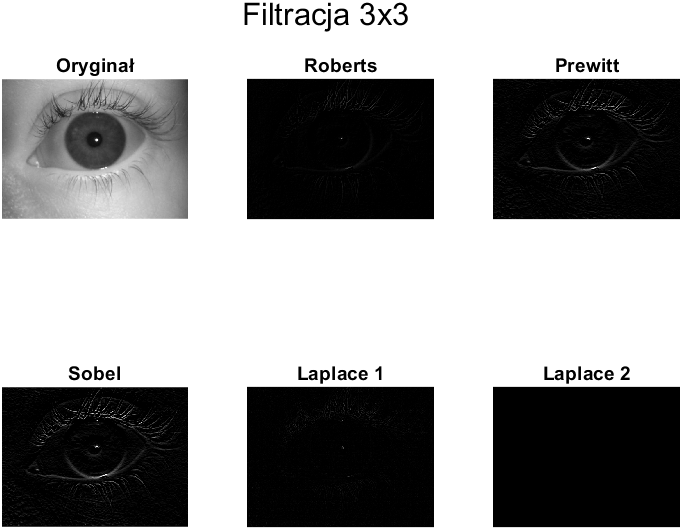
\includegraphics[width=\linewidth]{src/Lab002/zadanie1images/filtracja_3x3.png}
		\caption{Filtracja splotowa 3x3}
		\label{fig:3x3}
	\end{subfigure}
	\hfill
	\begin{subfigure}[t]{0.45\linewidth}
		\centering
		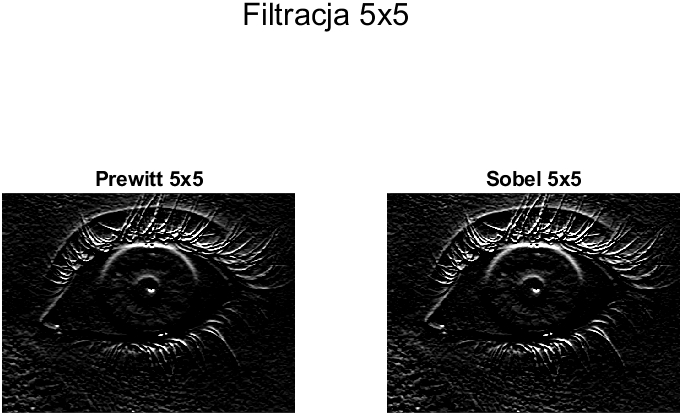
\includegraphics[width=\linewidth]{src/Lab002/zadanie1images/filtracja_5x5.png}
		\caption{Filtracja splotowa 5x5}
		\label{fig:5x5}
	\end{subfigure}

	\begin{subfigure}[t]{0.45\linewidth}
		\centering
		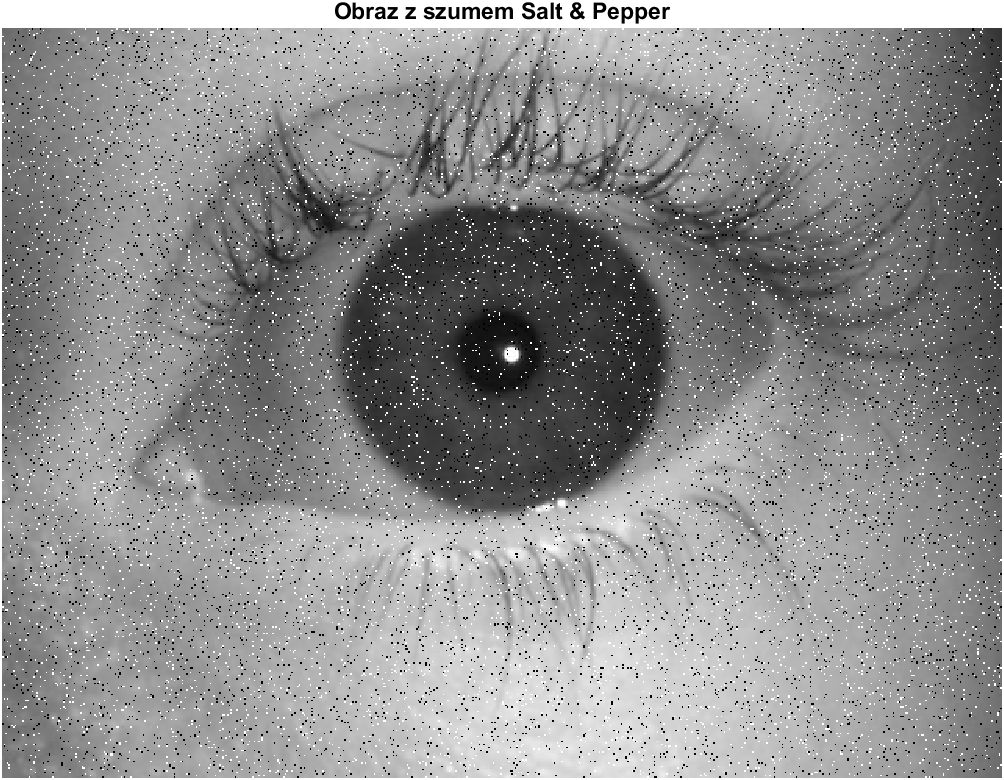
\includegraphics[width=\linewidth]{src/Lab002/zadanie1images/szum_salt_pepper.png}
		\caption{Obraz z szumem Salt and Pepper}
		\label{fig:SaltNPepper}
	\end{subfigure}
	\hfill
	\begin{subfigure}[t]{0.45\linewidth}
		\centering
		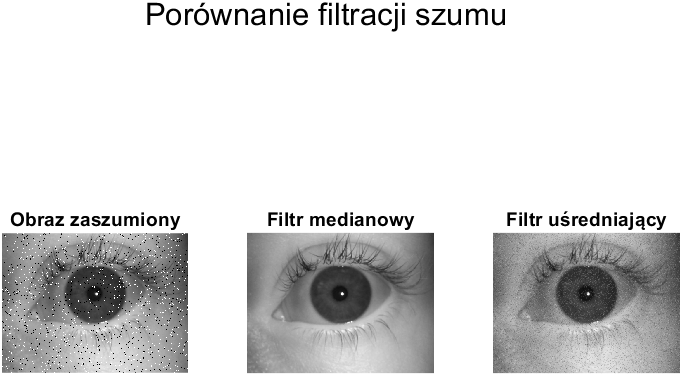
\includegraphics[width=\linewidth]{src/Lab002/zadanie1images/filtracja_szumu.png}
		\caption{Filtracja medianowa i uśredniająca}
		\label{fig:filteringMU}
	\end{subfigure}
	
	\begin{subfigure}[t]{0.45\linewidth}
		\centering
		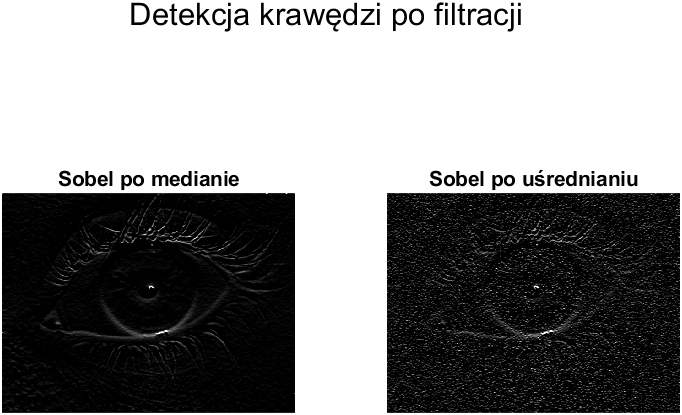
\includegraphics[width=\linewidth]{src/Lab002/zadanie1images/detekcja_krawedzi_po_filtracji.png}
		\caption{Detekja po filtracji}
		\label{fig:AfterFiltering}
	\end{subfigure}
	\hfill
	\begin{subfigure}[t]{0.45\linewidth}
		\centering
		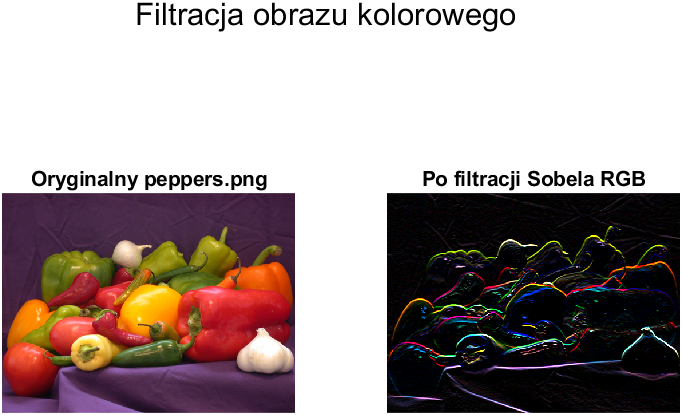
\includegraphics[width=\linewidth]{src/Lab002/zadanie1images/filtracja_rgb.png}
		\caption{Filtracja obrazu kolorowego}
		\label{fig:filtracja_rgb}
	\end{subfigure}

	\begin{subfigure}[t]{0.45\linewidth}
		\centering
		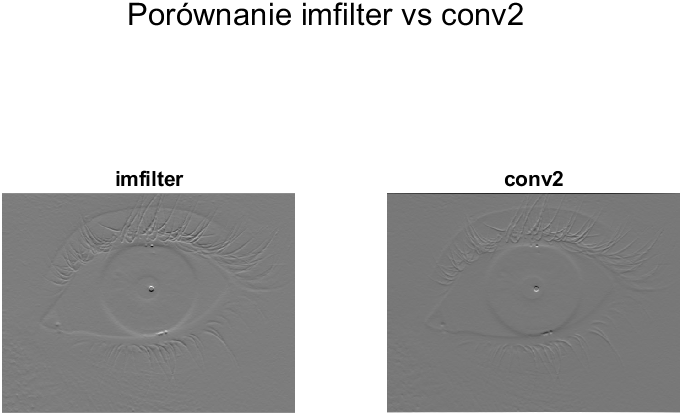
\includegraphics[width=\linewidth]{src/Lab002/zadanie1images/porownanie_imfilter_conv2.png}
		\caption{Porównanie imfilter i conv2}
		\label{fig:Imfilter_Conv2}
	\end{subfigure}
	
	\caption{Wizualizacja obrazów w różnych filtracjach splotowych.}
	\label{fig:lab002_images1}
\end{figure}

\section{Wnioski}
Na podstawie przeprowadzonych eksperymentów można stwierdzić, że:

\begin{itemize}
	\item \textbf{Filtry krawędziowe (Roberts, Prewitt, Sobel, Laplace)} skutecznie wykrywają zmiany intensywności w obrazie, jednak ich charakterystyka znacząco się różni. Operator Robertsa jest prosty i szybki obliczeniowo, lecz wykazuje dużą wrażliwość na szum i słabo radzi sobie z krawędziami innymi niż ukośne. Operator Prewitta oraz Sobela są bardziej odpornymi filtrami, przy czym filtr Sobela oferuje lepsze wygładzenie dzięki większemu obciążeniu środkowych pikseli. Operator Laplace’a umożliwia wykrycie krawędzi niezależnie od kierunku, ale jego wrażliwość na szumy jest jeszcze większa niż filtrów pierwszorzędowych.
	
	\item \textbf{Rozmiar maski filtra} wpływa na wynik filtracji: maski 5x5 zapewniają mocniejsze wygładzanie i bardziej rozmyte krawędzie w porównaniu do masek 3x3. Zwiększenie rozmiaru maski powoduje, że filtr staje się mniej czuły na drobne detale i szum, ale za to mniej precyzyjnie lokalizuje krawędzie.
	
	\item \textbf{Wpływ szumu Salt\&Pepper} na jakość obrazu jest znaczny. Obecność tego typu zakłóceń prowadzi do licznych, losowych zaburzeń w obrazie, które mogą zostać błędnie zinterpretowane jako krawędzie podczas procesu filtracji.
	
	\item \textbf{Filtr medianowy} wykazuje wysoką skuteczność w usuwaniu szumu typu Salt\&Pepper przy zachowaniu krawędzi oraz struktury obrazu. W przeciwieństwie do niego, \textbf{filtr uśredniający} rozmywa obraz, prowadząc do rozmycia granic i mniejszej skuteczności w eliminacji impulsowych zakłóceń.
	
	\item \textbf{Filtracja obrazu kolorowego} (na osobnych kanałach RGB) umożliwia skuteczne przetwarzanie obrazów wielokanałowych. Jednak filtracja niezależnie każdego kanału może prowadzić do powstania artefaktów kolorystycznych, zwłaszcza w obszarach o silnych zmianach koloru.
	
	\item \textbf{Porównanie funkcji imfilter oraz conv2} wykazało, że obie metody dają podobne wyniki przy odpowiednim doborze opcji (parametr \texttt{'same'}). Funkcja \texttt{imfilter} jest bardziej elastyczna, oferując możliwość wyboru metody obsługi brzegów obrazu oraz zachowania typu danych. Z kolei \texttt{conv2} jest bardziej „surowa” i wymaga ręcznego dostosowania typu i rozmiaru wyniku.
\end{itemize}

Podsumowując, odpowiedni dobór metody filtracji, rozmiaru maski oraz sposobu redukcji szumów ma kluczowe znaczenie dla skutecznej analizy obrazów biometrycznych i przetwarzania obrazów cyfrowych w ogóle.

\chapter{Laboratorium 3}
\label{cha:Lab003}
\makeatletter


% *********************************************************************
% w poniższej metryczce należy uzupełnić informacje o:
% - temacie ćwiczenia
% - numer ćwiczenia
% - numer grupy laboratoryjnej
% - numer zespołu
% - datę wykonania ćwiczenia oraz oddania ćwiczenia.
% *********************************************************************

\begin{table}[H]
    \centering
    \renewcommand{\tabularxcolumn}[1]{m{#1}}  % Dostosowanie kolumny do zawartości
    \newcolumntype{C}{>{\centering\arraybackslash}X}
    \begin{tabularx}{\linewidth}{|C|C|}
        \hline
        \multicolumn{2}{|c|}{\makecell{\textbf{\Large{Biometryczne Systemy Zabezpieczeń}} \\ \textbf{Ćwiczenia Laboratoryjne}}} \\ \hline
        \multicolumn{1}{|l|}{Temat}                    &              OPERACJE MORFOLOGICZNE NA OBRAZACH            \\ \hline
        \multicolumn{1}{|l|}{Ćwiczenie nr:}                    &      03                   \\ \hline
        \multicolumn{1}{|l|}{Autorzy:}                         &   \@author                              \\ \hline
        \multicolumn{1}{|l|}{Grupa laboratoryjna}                       &       02               \\ \hline
        \multicolumn{1}{|l|}{Zespół nr. }                       &    XX                  \\ \hline
        \multicolumn{1}{|l|}{Data wykonana ćwiczenia}         &  26.04.2025     \\ \hline
        \multicolumn{1}{|l|}{Data oddania ćwiczenia  }         &   13.05.2025     \\ \hline
    \end{tabularx}
\end{table}


\section{Cel ćwiczenia}

Operacje morfologiczne są kluczowym narzędziem w przetwarzaniu obrazów, szczególnie w analizie
kształtów i struktury obiektów. Dzięki wykorzystaniu odpowiednich elementów strukturalnych można
dostosować te operacje do różnych zadań, takich jak segmentacja, poprawa jakości obrazu czy analiza
konturów. Celem laboratorium jest zapoznanie się z operacjami morfologicznymi na obrazach.

\section{Wstęp teoretyczny}

Operacje morfologiczne to techniki przetwarzania obrazów stosowane głównie do analizy kształtu i struktury obiektów w obrazach binarnych oraz, w pewnym stopniu, w obrazach w skali szarości. Ich główną cechą jest wykorzystanie elementów strukturalnych do modyfikowania obrazu.

\textbf{Szkieletyzacja} to proces odnoszący się do ścieniania linii konturowych obiektu, który znalazł zastosowanie w wielu dziedzinach, takich jak:
\begin{itemize}
	\item medycyna (analiza białych ciałek krwi, chromosomów, naczyń wieńcowych),
	\item kryminalistyka (rozpoznawanie odcisków palców),
	\item przemysł elektroniczny (analiza obwodów drukowanych),
	\item wektoryzacja obrazów rastrowych.
\end{itemize}

W niniejszym opracowaniu przedstawiono sposób działania wybranych algorytmów szkieletyzujących: Arcelli-Levialdi-Pavlidis, Chin-Van-Stover-Iverson oraz Rosenfeld-Peleg. Zaprojektowano także aplikację umożliwiającą użytkownikowi wprowadzanie własnych szablonów szkieletyzujących oraz obserwowanie otrzymanych wyników.

\subsection{Szkieletyzacja obrazów binarnych}

Spośród klasycznych metod ścieniania (\textit{skeletoning} lub \textit{thinning algorithms}), wyróżnić można trzy główne podejścia:
\begin{itemize}
	\item \textbf{Wypełnianie działów wodnych} (dla obrazów w skali szarości),
	\item \textbf{Hit or Miss Transform} (dla obrazów binarnych i szarych),
	\item \textbf{Medial Axis Transform} (posiadająca przekształcenie odwrotne).
\end{itemize}

Podstawą tych metod są dwa główne przekształcenia morfologiczne: erozja i dylatacja. Formalnie, dla obrazów binarnych:

\begin{equation}
	A \oplus B = \bigcup_{b \in B} \left( \bigcup_{a \in A} (a + b) \right)
\end{equation}

\begin{equation}
	A \ominus B = \bigcap_{b \in B} \left( \bigcup_{a \in A} (a + b) \right)
\end{equation}

gdzie $A$ to obraz, $B$ to maska (element strukturalny), $\oplus$ oznacza dylatację, a $\ominus$ erozję. Znak $\bigcup$ oznacza sumę zbiorów, a $\bigcap$ ich część wspólną.

Hit or Miss Transform można opisać następująco:
\begin{itemize}
	\item przykładamy element strukturalny $b$ do każdego punktu obrazu,
	\item jeśli $b$ pokrywa się z sąsiedztwem - zmieniamy wartość piksela (zwykle na 0),
	\item w przeciwnym wypadku piksel pozostaje niezmieniony.
\end{itemize}

Algorytmy takie jak Arcelli-Levialdi stosują szablony operujące na oknie bieżącego piksela oraz jego ośmiu sąsiadów. Możliwa jest także modyfikacja szablonów (np. użycie bitów typu "don't care") w celu uzyskania lepszego efektu szkieletyzacji gałęzi pionowych.

\subsection{Algorytm Chin-Van-Stover-Iverson}

Algorytm CVSI porównuje sąsiedztwo piksela z zestawem szablonów (1--8). Jeśli spełniony jest warunek zgodności z szablonem, następuje dodatkowe porównanie z szablonami 9 i 10. 

\begin{itemize}
	\item Jeśli otoczenie nie różni się od żadnego z szablonów — piksel pozostaje (jest częścią szkieletu).
	\item Jeśli różni się — piksel zostaje usunięty.
\end{itemize}

Aplikacja umożliwia ręczną edycję szablonów przez użytkownika (zmiana wartości 0, 1, x za pomocą kliknięć).

\subsection{Szkieletyzacja obrazów tonowanych}

Naturalnym rozwinięciem szkieletyzacji obrazów binarnych jest szkieletyzacja obrazów w skali szarości. Przykładowe podejścia:

\begin{itemize}
	\item erozja (Rosenfeld-Peleg),
	\item przekształcenie typu top-hat.
\end{itemize}

Ogólna translacja sygnału $f(x)$:

\begin{equation}
	f(x) = f(x - z)
\end{equation}

\begin{equation}
	(f \oplus y)(x) = f(x) + y
\end{equation}

Obie translacje można łączyć:

\begin{equation}
	(f_z \oplus y)(x) = f(x - z) + y
\end{equation}

Jeśli przyjmiemy, że $f(x) = -\infty$ poza obrazem, to dziedzinę obrazu określimy jako:

\begin{equation}
	D[f] = \{x : f(x) > -\infty\}
\end{equation}

Jeżeli $g(x) \leq f(x)$ dla każdego $x$, to:

\begin{equation}
	D[g] \subseteq D[f]
\end{equation}

Erozję definiujemy jako:

\begin{equation}
	(f \wedge g)(x) = 
	\begin{cases}
		\min\{f(x), g(x)\}, & x \in D[f] \cap D[g] \\
		-\infty, & \text{inaczej}
	\end{cases}
\end{equation}

Przy zastosowaniu płaskiego elementu strukturyzującego ($g_z(x) = 0$), erozję można zapisać jako:

\begin{equation}
	(f \ominus g)(x) = \min\{f(x) - g_z(x)\}
\end{equation}

co odpowiada filtracji typu \textit{moving minimum}.

Do obserwacji zachowania algorytmu Rosenfeld-Peleg zaprojektowano obraz syntetyczny zawierający cylindryczną falę sinusoidalną.

\section{Zadania do wykonania samodzielnego}

\subsection{Zadanie 1}

\subsubsection{Treść}

\begin{enumerate}
	\item Załaduj obraz testowy oraz przygotuj obraz do realizacji dalszych ćwiczeń o rozmiarach:
	\item Wykonaj program realizujący algorytm ścieniania, którego zestaw kerneli zamieszczono poniżej:
	\item Do zaprogramowania kolejnych szablonów i masek wykorzystaj poniższy fragment kodu źródłowego (funkcja intbin8 formuje 8-bitową reprezentację liczby dziesiętnej przekazywanej parametrem i):
	\item Sprawdź poprawność działania algorytmu na innym obrazie testowym, dla zmodyfikowanych
	parametrów filtracji morfologicznej jak poniżej:
	\item Wyświetl wyniki otrzymanych filtracji wraz z podpisem w oknie wykorzystując funkcję subplot.
	\item Wyjaśnij zjawisko zmieniającej się szybkości wykonywania algorytmu w zależności od fazy jego wykonywania.
	\item Wykonaj wersję algorytmu realizującego szkieletyzację wg Chin-Wan-Stover-Iverson, przyjmując zestaw kerneli jak poniżej
	\item Przeprowadź dyskusję otrzymanych wyników jak dla pkt 5-6.
\end{enumerate}

\subsubsection{Przykładowy program}

\lstinputlisting[style= matlabStyle, caption= Wczytanie obrazu i stworzenie konwersji, label=Lab003_l1]{src/Lab003/zadanie1.m}

\subsubsection{Obrazy}

\begin{figure}[H]
	\centering
	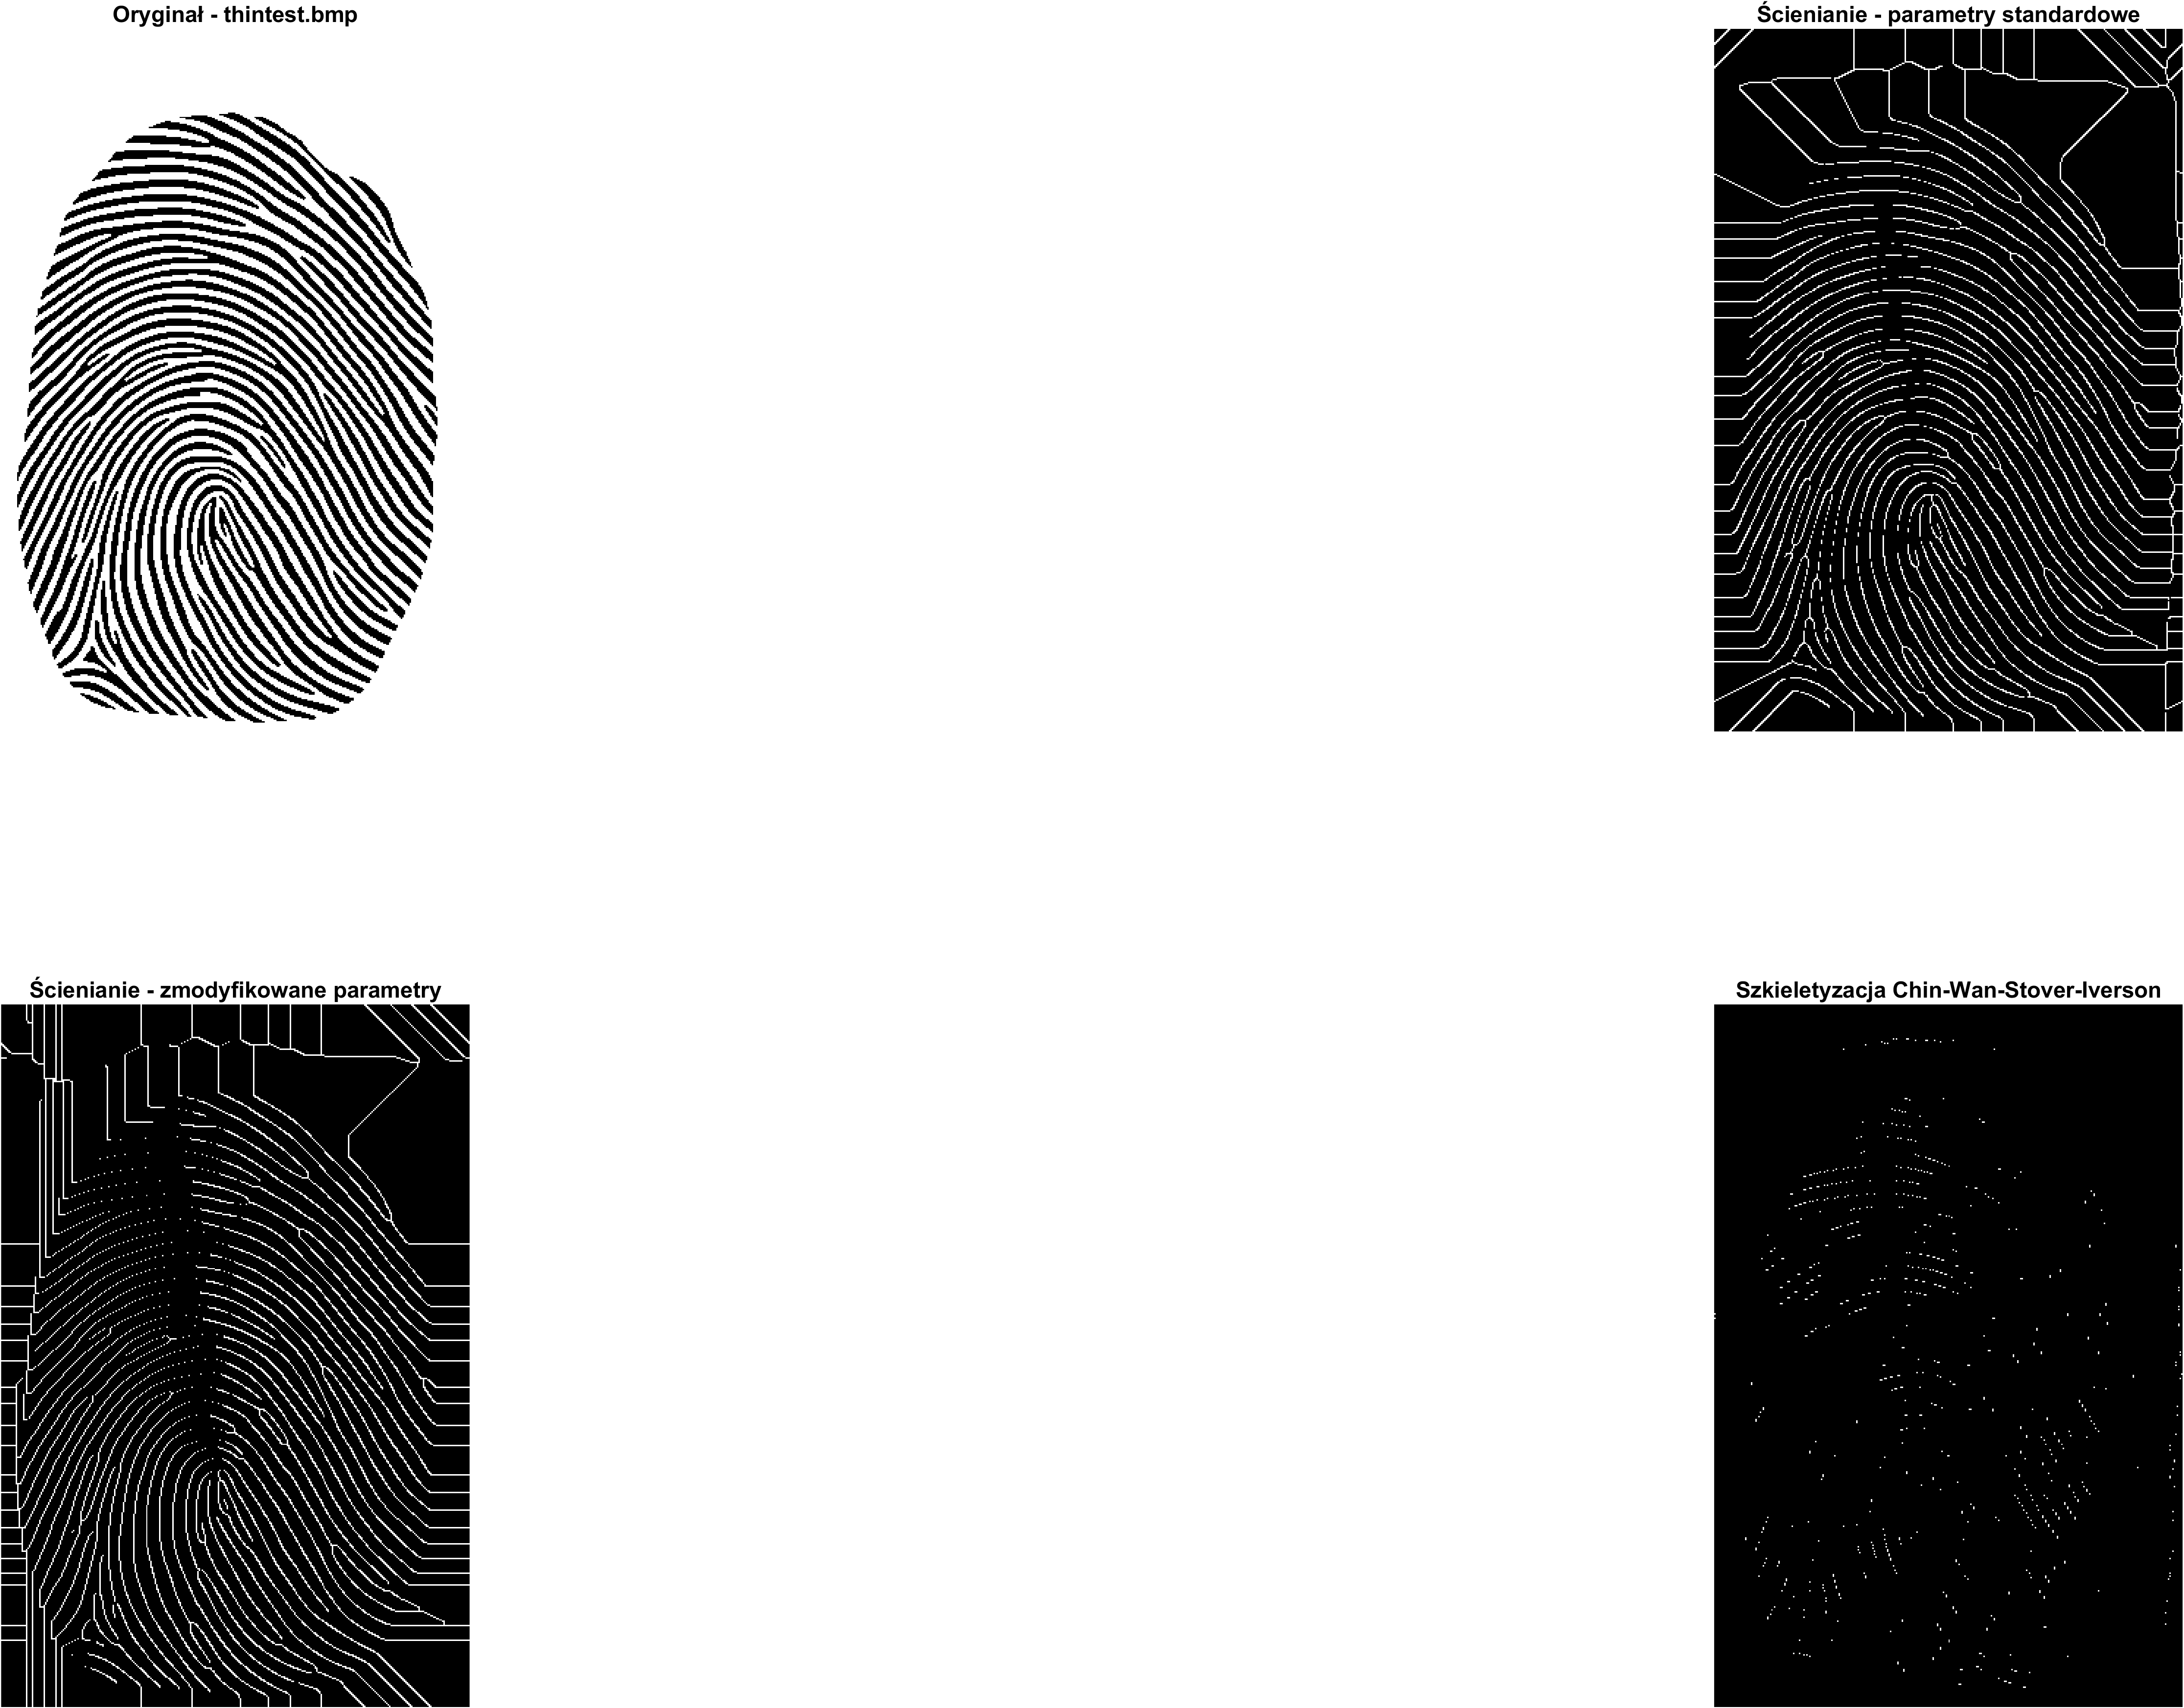
\includegraphics[width=0.8\textwidth]{src/Lab003/results.png}
	\caption{Porównanie wyników: Oryginał, Ścienianie standardowe, Ścienianie zmodyfikowane, Szkieletyzacja CWSI.}
\end{figure}

\section{Wnioski}

W przeprowadzonym ćwiczeniu dokonano analizy działania dwóch metod ścieniania obrazów binarnych:

\begin{itemize}
	\item Metody klasycznej ścieniania z wykorzystaniem standardowych oraz zmodyfikowanych masek.
	\item Metody szkieletyzacji Chin-Wan-Stover-Iverson.
\end{itemize}

Na podstawie uzyskanych wyników można wyciągnąć następujące wnioski:

\begin{enumerate}
	\item \textbf{Ścienianie z maskami standardowymi} pozwala na sukcesywne usuwanie zbędnych pikseli z obrazu, prowadząc do uzyskania cieńszych struktur. Proces ten jest stosunkowo stabilny, zachowując kształt linii papilarnych.
	
	\item \textbf{Zmodyfikowane parametry ścieniania} powodują bardziej agresywne usuwanie pikseli. Widoczne jest zwiększone uproszczenie obrazu, jednak miejscami może to prowadzić do zniekształcenia struktury oryginalnych linii.
	
	\item \textbf{Szkieletyzacja metodą Chin-Wan-Stover-Iverson} skutkuje szybkim i skutecznym redukowaniem obrazu do jego podstawowych konturów. Uzyskany szkielet jest bardzo cienki, jednak często prowadzi do fragmentacji obrazu, zwłaszcza w miejscach o większej gęstości pikseli.
	
	\item \textbf{Szybkość działania algorytmu} jest największa na początku, gdy usuwane są większe grupy pikseli. W późniejszych iteracjach proces znacznie zwalnia, ponieważ zmiany obejmują pojedyncze piksele.
	
	\item Obie metody pozwalają na skuteczne ścienianie obrazów binarnych, jednak wybór odpowiedniej metody oraz parametrów powinien być dostosowany do specyfiki przetwarzanego obrazu oraz wymagań aplikacji końcowej (np. analizy odcisków palców, rozpoznawania wzorców itp.).
\end{enumerate}

Dzięki zastosowaniu różnych wariantów masek oraz metod możliwe jest dostosowanie procesu ścieniania do indywidualnych potrzeb, co stanowi istotny aspekt w cyfrowym przetwarzaniu obrazów.
\chapter{Laboratorium 4}
\label{cha:Lab004}
\makeatletter


% *********************************************************************
% w poniższej metryczce należy uzupełnić informacje o:
% - temacie ćwiczenia
% - numer ćwiczenia
% - numer grupy laboratoryjnej
% - numer zespołu
% - datę wykonania ćwiczenia oraz oddania ćwiczenia.
% *********************************************************************

\begin{table}[H]
    \centering
    \renewcommand{\tabularxcolumn}[1]{m{#1}}  % Dostosowanie kolumny do zawartości
    \newcolumntype{C}{>{\centering\arraybackslash}X}
    \begin{tabularx}{\linewidth}{|C|C|}
        \hline
        \multicolumn{2}{|c|}{\makecell{\textbf{\Large{Biometryczne Systemy Zabezpieczeń}} \\ \textbf{Ćwiczenia Laboratoryjne}}} \\ \hline
        \multicolumn{1}{|l|}{Temat}                    &             TRANSFORMATA HOUGHA            \\ \hline
        \multicolumn{1}{|l|}{Ćwiczenie nr:}                    &      04                   \\ \hline
        \multicolumn{1}{|l|}{Autorzy:}                         &   \@author                              \\ \hline
        \multicolumn{1}{|l|}{Grupa laboratoryjna}                       &       02               \\ \hline
        \multicolumn{1}{|l|}{Zespół nr. }                       &    XX                  \\ \hline
        \multicolumn{1}{|l|}{Data wykonana ćwiczenia}         &  27.04.2025     \\ \hline
        \multicolumn{1}{|l|}{Data oddania ćwiczenia  }         &   13.05.2025     \\ \hline
    \end{tabularx}
\end{table}

\section{Cel ćwiczenia}

Celem zajęć jest zapoznanie się z transformacją Hough’a w zadaniu wykrywania linii i okręgów
w testowych obrazach binarnych oraz obrazach tonowanych pozyskiwanych ze skanerów tęczówki
oka.

\section{Wstęp teoretyczny}

\section{Opis wykorzystywanego oprogramowania i narzędzi}

\section{Zadania do wykonania samodzielnego}

\subsection{Zadanie1 }

\subsubsection{Treść}


\subsubsection{Przykładowy program}

\subsubsection{Obrazy}

\section{Wnioski}

\subsection{Zadanie X}

\subsubsection{Treść}

\subsubsection{Przykładowy program}

\subsubsection{Obrazy}

\section{Wnioski}

Na podstawie przeprowadzonych eksperymentów można stwierdzić, że:
\chapter{Laboratorium 5}
\label{cha:Lab005}
\makeatletter


% *********************************************************************
% w poniższej metryczce należy uzupełnić informacje o:
% - temacie ćwiczenia
% - numer ćwiczenia
% - numer grupy laboratoryjnej
% - numer zespołu
% - datę wykonania ćwiczenia oraz oddania ćwiczenia.
% *********************************************************************

\begin{table}[H]
    \centering
    \renewcommand{\tabularxcolumn}[1]{m{#1}}  % Dostosowanie kolumny do zawartości
    \newcolumntype{C}{>{\centering\arraybackslash}X}
    \begin{tabularx}{\linewidth}{|C|C|}
        \hline
        \multicolumn{2}{|c|}{\makecell{\textbf{\Large{Biometryczne Systemy Zabezpieczeń}} \\ \textbf{Ćwiczenia Laboratoryjne}}} \\ \hline
        \multicolumn{1}{|l|}{Temat}                    &              TRANSFORMATA FOURIERA, CZĘSTOTLIWOŚCIOWA ANALIZA OBRAZU            \\ \hline
        \multicolumn{1}{|l|}{Ćwiczenie nr:}                    &      05                   \\ \hline
        \multicolumn{1}{|l|}{Autorzy:}                         &   \@author                              \\ \hline
        \multicolumn{1}{|l|}{Grupa laboratoryjna}                       &       02               \\ \hline
        \multicolumn{1}{|l|}{Zespół nr. }                       &    XX                  \\ \hline
        \multicolumn{1}{|l|}{Data wykonana ćwiczenia}         &  05.05.2025     \\ \hline
        \multicolumn{1}{|l|}{Data oddania ćwiczenia  }         &   13.05.2025     \\ \hline
    \end{tabularx}
\end{table}


\section{Cel ćwiczenia}

Transformata Fouriera (TF) to jedno z podstawowych narzędzi w analizie sygnałów i obrazów, które
pozwala na przejście z dziedziny przestrzennej do dziedziny częstotliwościowej. Dzięki temu można
analizować, jak różne składowe częstotliwościowe wpływają na obraz i stosować różne techniki filtracji.
W laboratorium przenalizowane będą informacje związane z obliczaniem transformaty Fouriera
obrazu, wizualizacji jego widma częstotliwościowego oraz stosowane operacje filtracji.

\section{Wstęp teoretyczny}

Transformata Fouriera to jedno z podstawowych narzędzi analizy sygnałów i obrazów. Dzięki niej możliwe jest przejście z dziedziny przestrzennej (lub czasowej) do dziedziny częstotliwościowej, co umożliwia identyfikację ukrytych struktur, analizę filtracji oraz kompresji danych. W przypadku obrazów cyfrowych stosuje się dwuwymiarową wersję transformaty Fouriera – 2D DFT (Discrete Fourier Transform).

Dyskretna transformata Fouriera (DFT) dla obrazu dwuwymiarowego $f(x, y)$ z rozmiarami $M \times N$ jest zdefiniowana jako:

\begin{equation}
	F(u, v) = \sum_{x=0}^{M-1} \sum_{y=0}^{N-1} f(x, y) \cdot e^{-j2\pi \left( \frac{ux}{M} + \frac{vy}{N} \right)}
\end{equation}

Natomiast transformata odwrotna, pozwalająca odtworzyć oryginalny obraz z jego reprezentacji częstotliwościowej, wyrażona jest wzorem:

\begin{equation}
	f(x, y) = \frac{1}{MN} \sum_{u=0}^{M-1} \sum_{v=0}^{N-1} F(u, v) \cdot e^{j2\pi \left( \frac{ux}{M} + \frac{vy}{N} \right)}
\end{equation}

W środowisku \textsc{Matlab}, do obliczania tych przekształceń służą wbudowane funkcje:
\begin{itemize}
	\item \texttt{fft2()} – oblicza dwuwymiarową szybką transformatę Fouriera,
	\item \texttt{ifft2()} – oblicza odwrotną dwuwymiarową transformację Fouriera.
\end{itemize}

Matematyczne podstawy transformaty Fouriera sięgają początku XIX wieku i są związane z pracą Jeana Baptiste'a Fouriera, który zaproponował, że każda funkcja okresowa spełniająca warunki Dirichleta może być przedstawiona jako suma sinusów i cosinusów:

\begin{equation}
	x(t) = a_0 + \sum_{n=1}^{\infty} \left( a_n \cos(n\omega_0 t) + b_n \sin(n\omega_0 t) \right)
\end{equation}

gdzie $T = \frac{2\pi}{\omega_0}$ oznacza okres funkcji.

Współczynniki $a_n$ i $b_n$ mają następujące własności:
\begin{itemize}
	\item Jeśli $x(t)$ jest funkcją parzystą, to $b_n = 0$,
	\item Jeśli $x(t)$ jest funkcją nieparzystą, to $a_n = 0$,
	\item Jeśli $x(t + T/2) = -x(t)$, to zanikają parzyste harmoniczne.
\end{itemize}

Współczynniki te można obliczyć jako:

\begin{align}
	a_0 &= \frac{1}{T} \int_0^T x(t) \,dt \\
	a_n &= \frac{2}{T} \int_0^T x(t) \cos(n\omega_0 t) \,dt \\
	b_n &= \frac{2}{T} \int_0^T x(t) \sin(n\omega_0 t) \,dt
\end{align}

Interaktywny przewodnik po transformacie Fouriera można znaleźć pod adresem: 
\url{https://www.jezzamon.com/fourier/pl.html} lub \url{https://github.com/Jezzamonn/fourier} (dostęp: 18.02.2025). 

Szczegółowe informacje teoretyczne na temat transformaty Fouriera dostępne są również na stronie: 
\url{https://home.agh.edu.pl/~zobmat/2020/II_mich_mar/index.html} (dostęp: 18.02.2025).


\section{Opis wykorzystywanego oprogramowania i narzędzi}


\section{Zadania do wykonania samodzielnego}

\subsection{Zadanie 1}

\subsubsection{Treść}

W oparciu o poniższy opis struktury algorytmu związanego z rozkładem w szereg Fouriera zaproponuj
jego implementację. Struktura algorytmu:

\begin{itemize}
	\item Inicjalizacja – zamknięcie otwartych okien, czyszczenie pamięci, ustawienie parametrów.
 	\item Generowanie funkcji wejściowej – tworzenie sygnału do analizy.
	\item Rozkład na harmoniczne – obliczanie współczynników Fouriera.
	\item Sumowanie składowych – rekonstrukcja funkcji.	
	\item Wizualizacja wyników – rysowanie wykresów poszczególnych harmonicznych i sygnałukońcowego.
\end{itemize}

\subsubsection{Przykładowy program}

\lstinputlisting[style= matlabStyle, caption= Algorytm rozkładu w szereg Fouriera, label=Lab005_l1]{src/Lab005/zadanie1.m}

\subsubsection{Obrazy}

\begin{figure}[H]
	\centering
	\begin{subfigure}[t]{0.45\linewidth}
		\centering
		
\includegraphics[width=\linewidth]{src/lab005/original.png}
		\label{fig:lab5z1_original}
	\end{subfigure}
	
	\centering
	\begin{subfigure}[t]{0.45\linewidth}
		\centering
		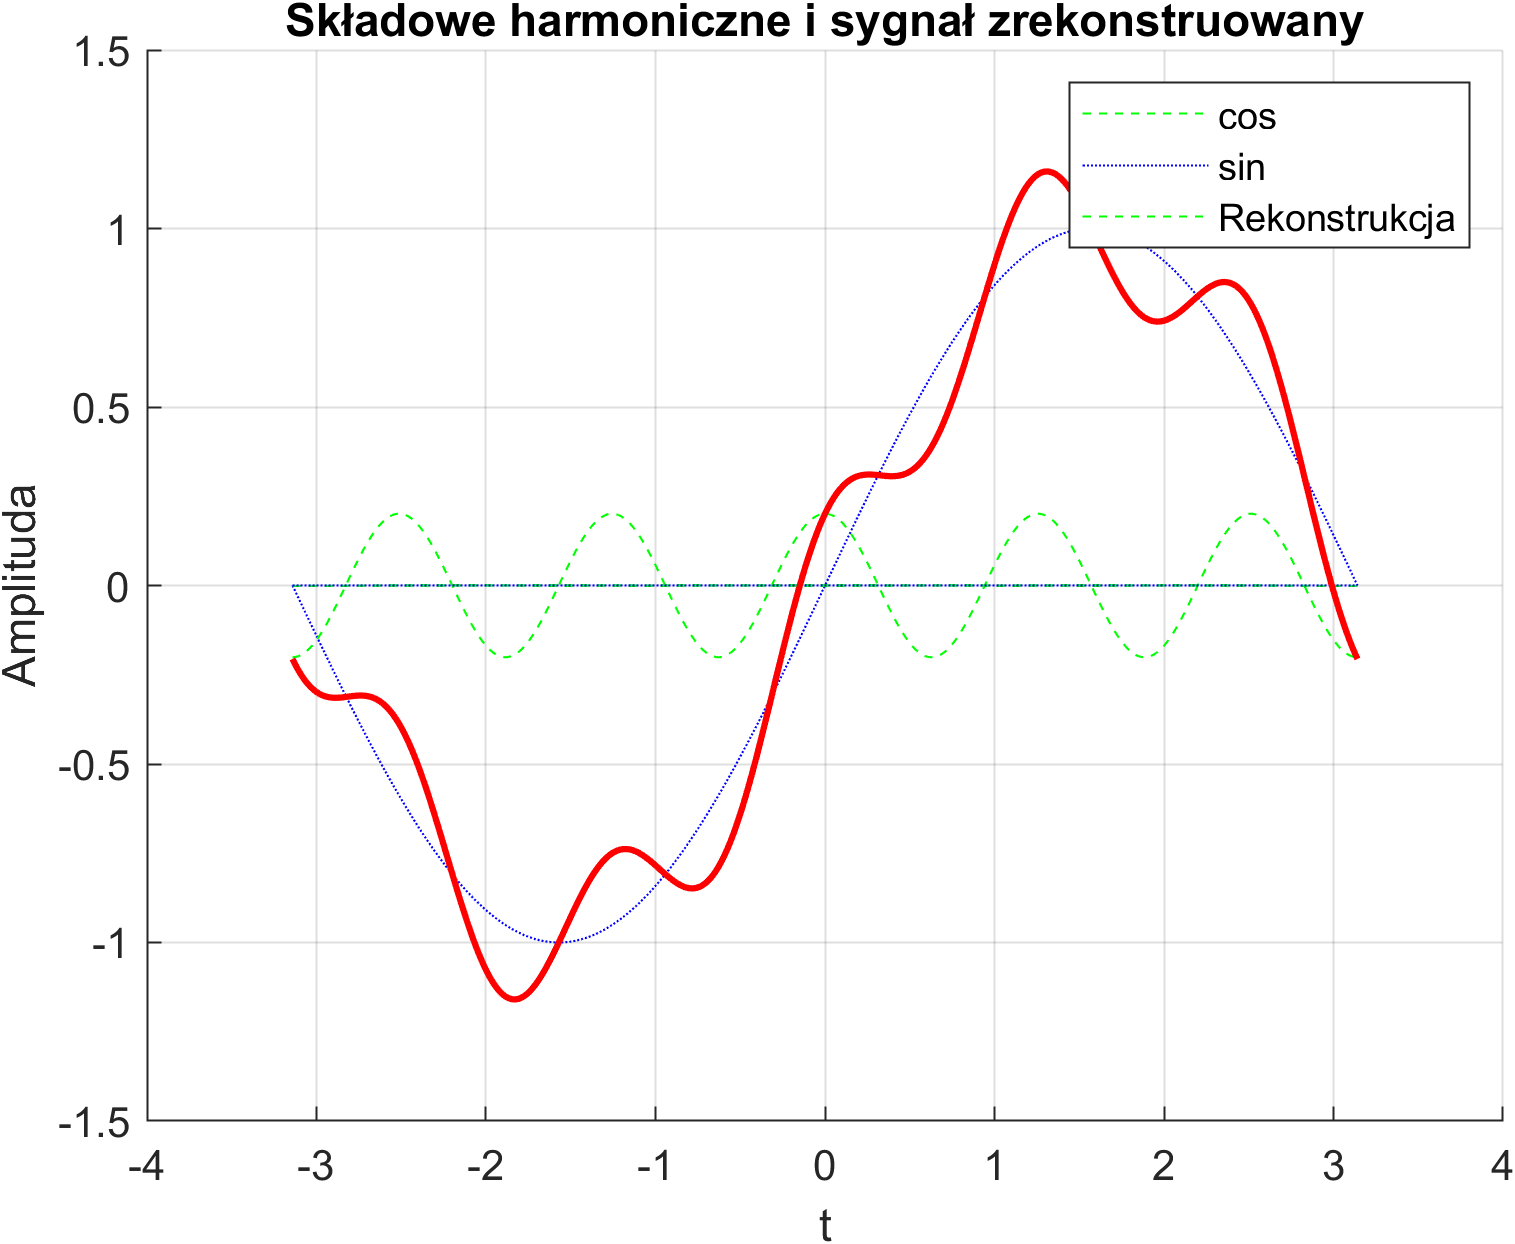
\includegraphics[width=\linewidth]{src/Lab005/recon_harmon.png}
		\label{fig:lab5z1_recon_harmon}
	\end{subfigure}
	\hfill
	\begin{subfigure}[t]{0.45\linewidth}
		\centering
		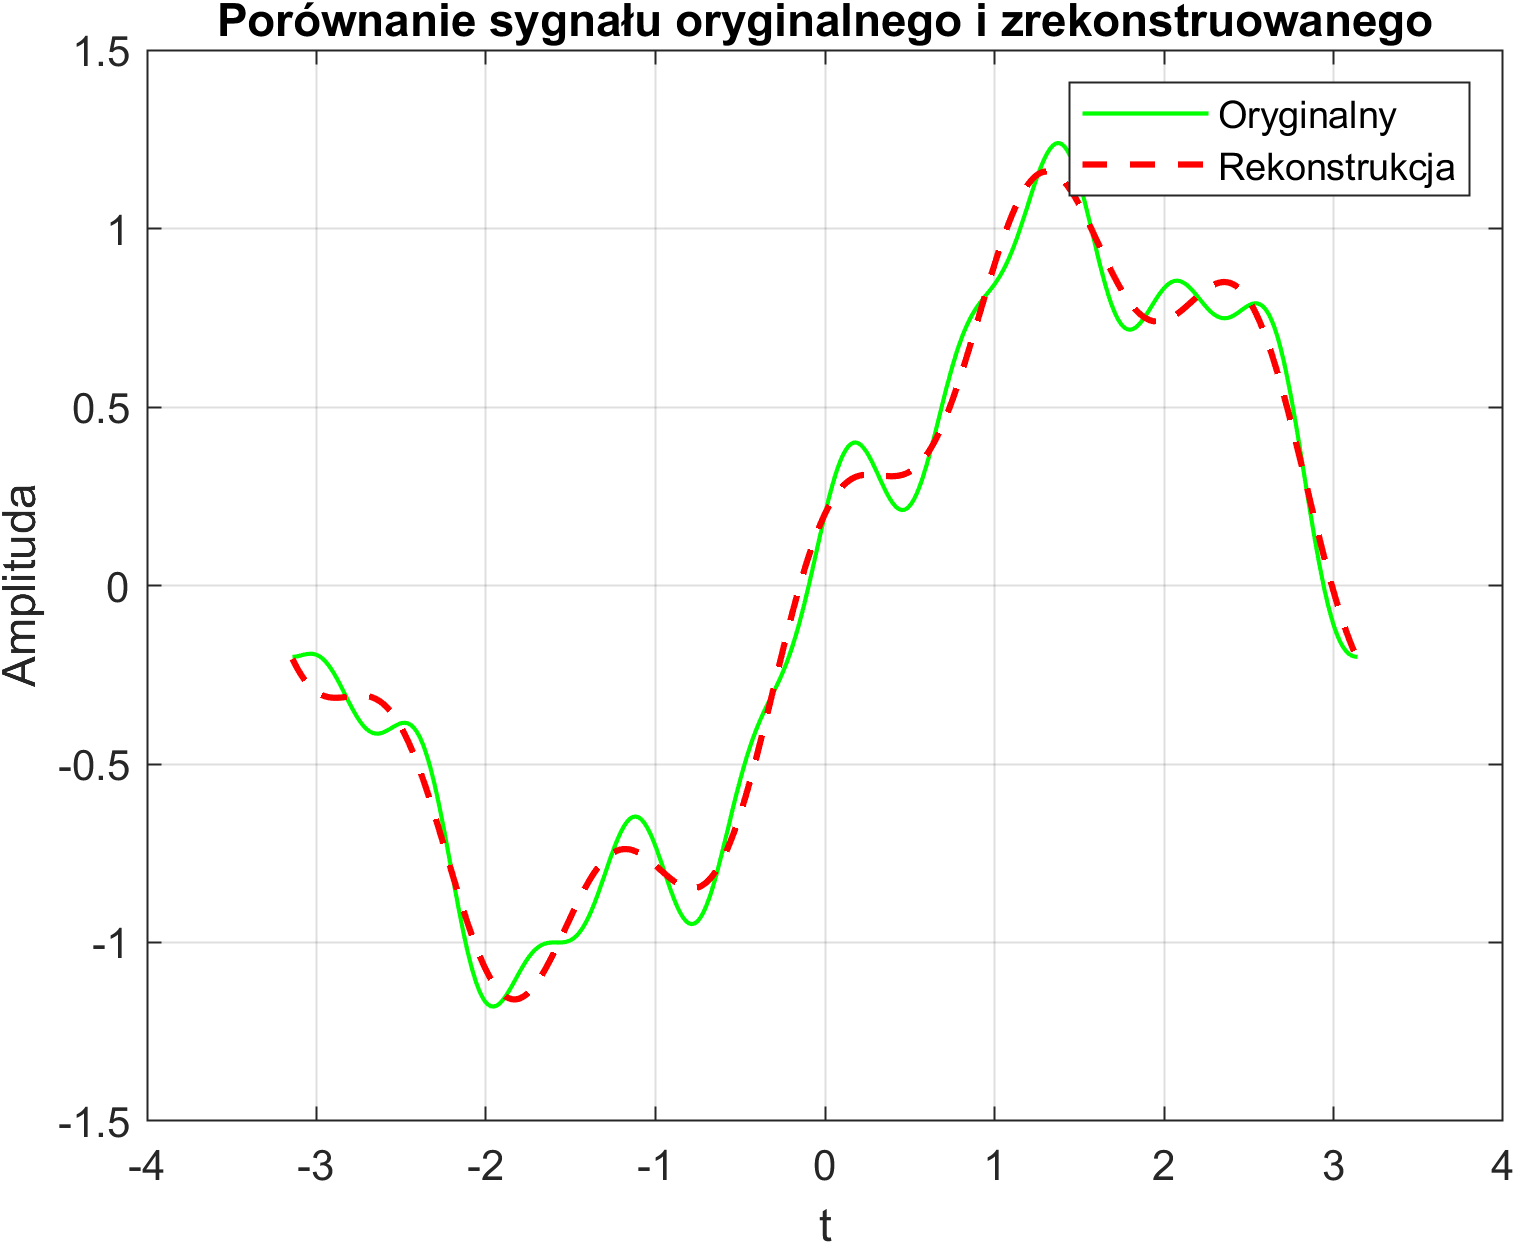
\includegraphics[width=\linewidth]{src/Lab005/comparison.png}
		\label{fig:lab5_comparison}
	\end{subfigure}
	
	\centering
	\begin{subfigure}[t]{0.45\linewidth}
		\centering
		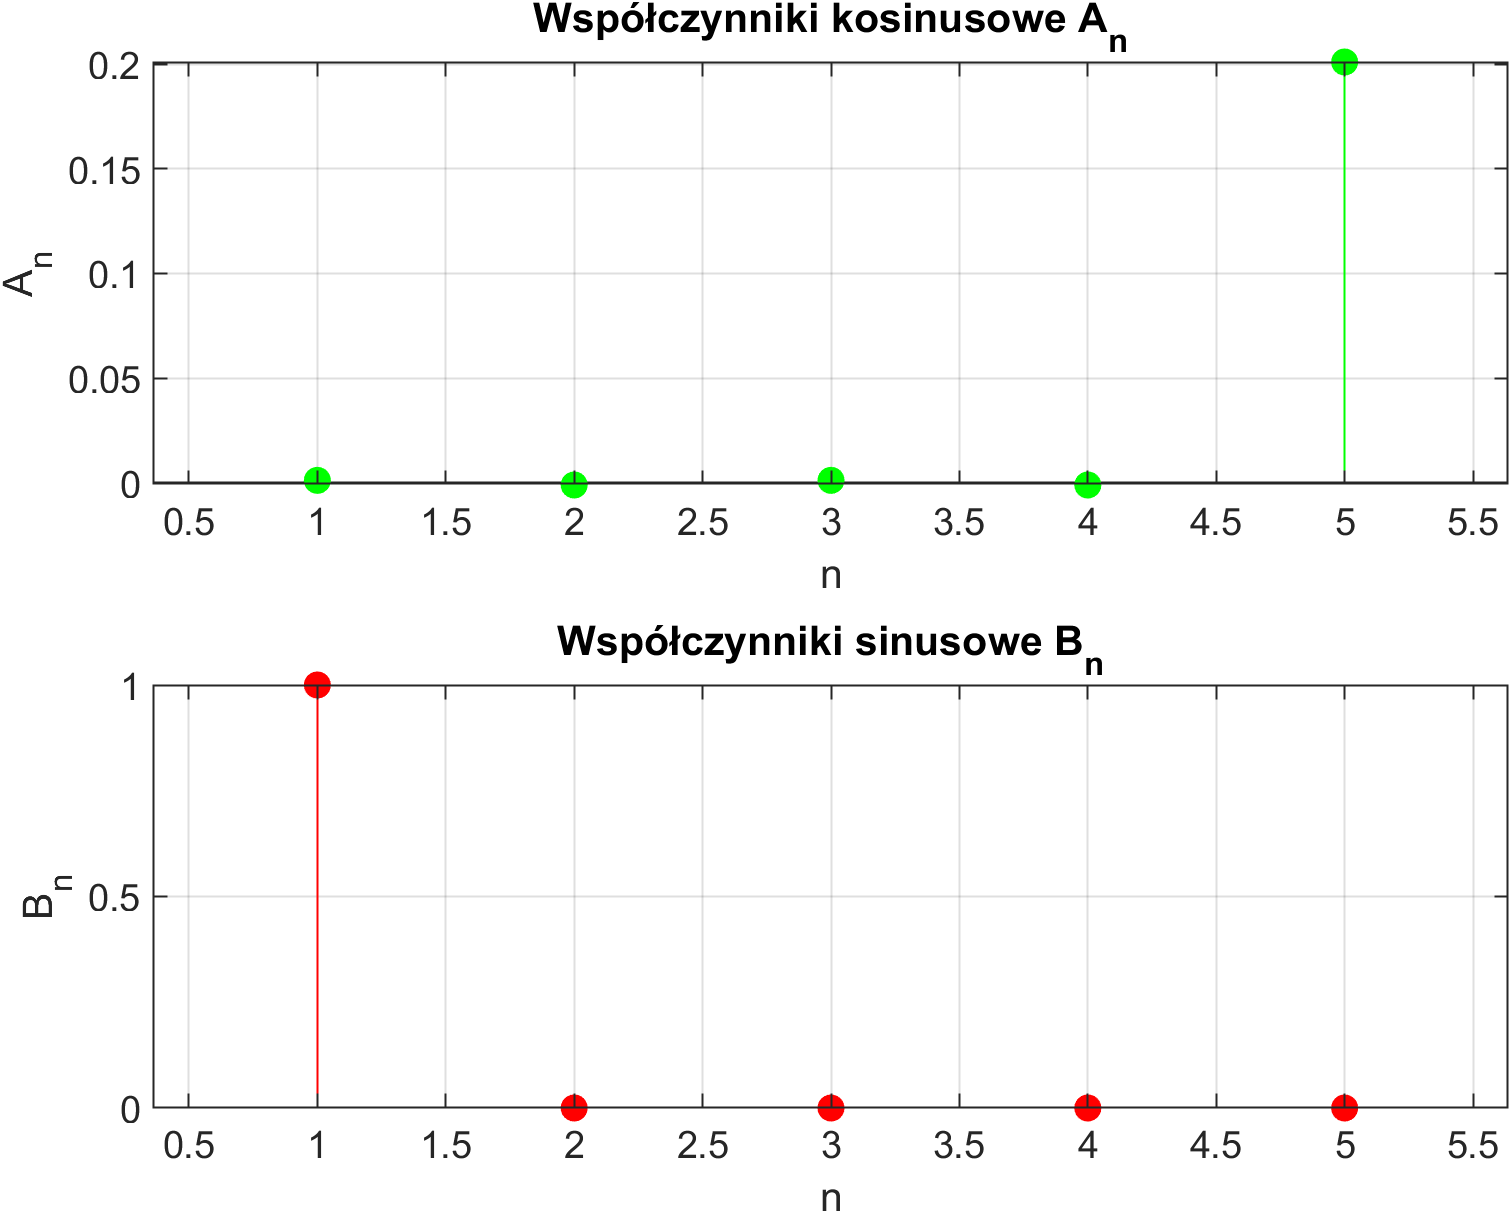
\includegraphics[width=\linewidth]{src/Lab005/coeff.png}
		\label{fig:lab5z1_coeff}
	\end{subfigure}
	\hfill
	\begin{subfigure}[t]{0.45\linewidth}
		\centering
		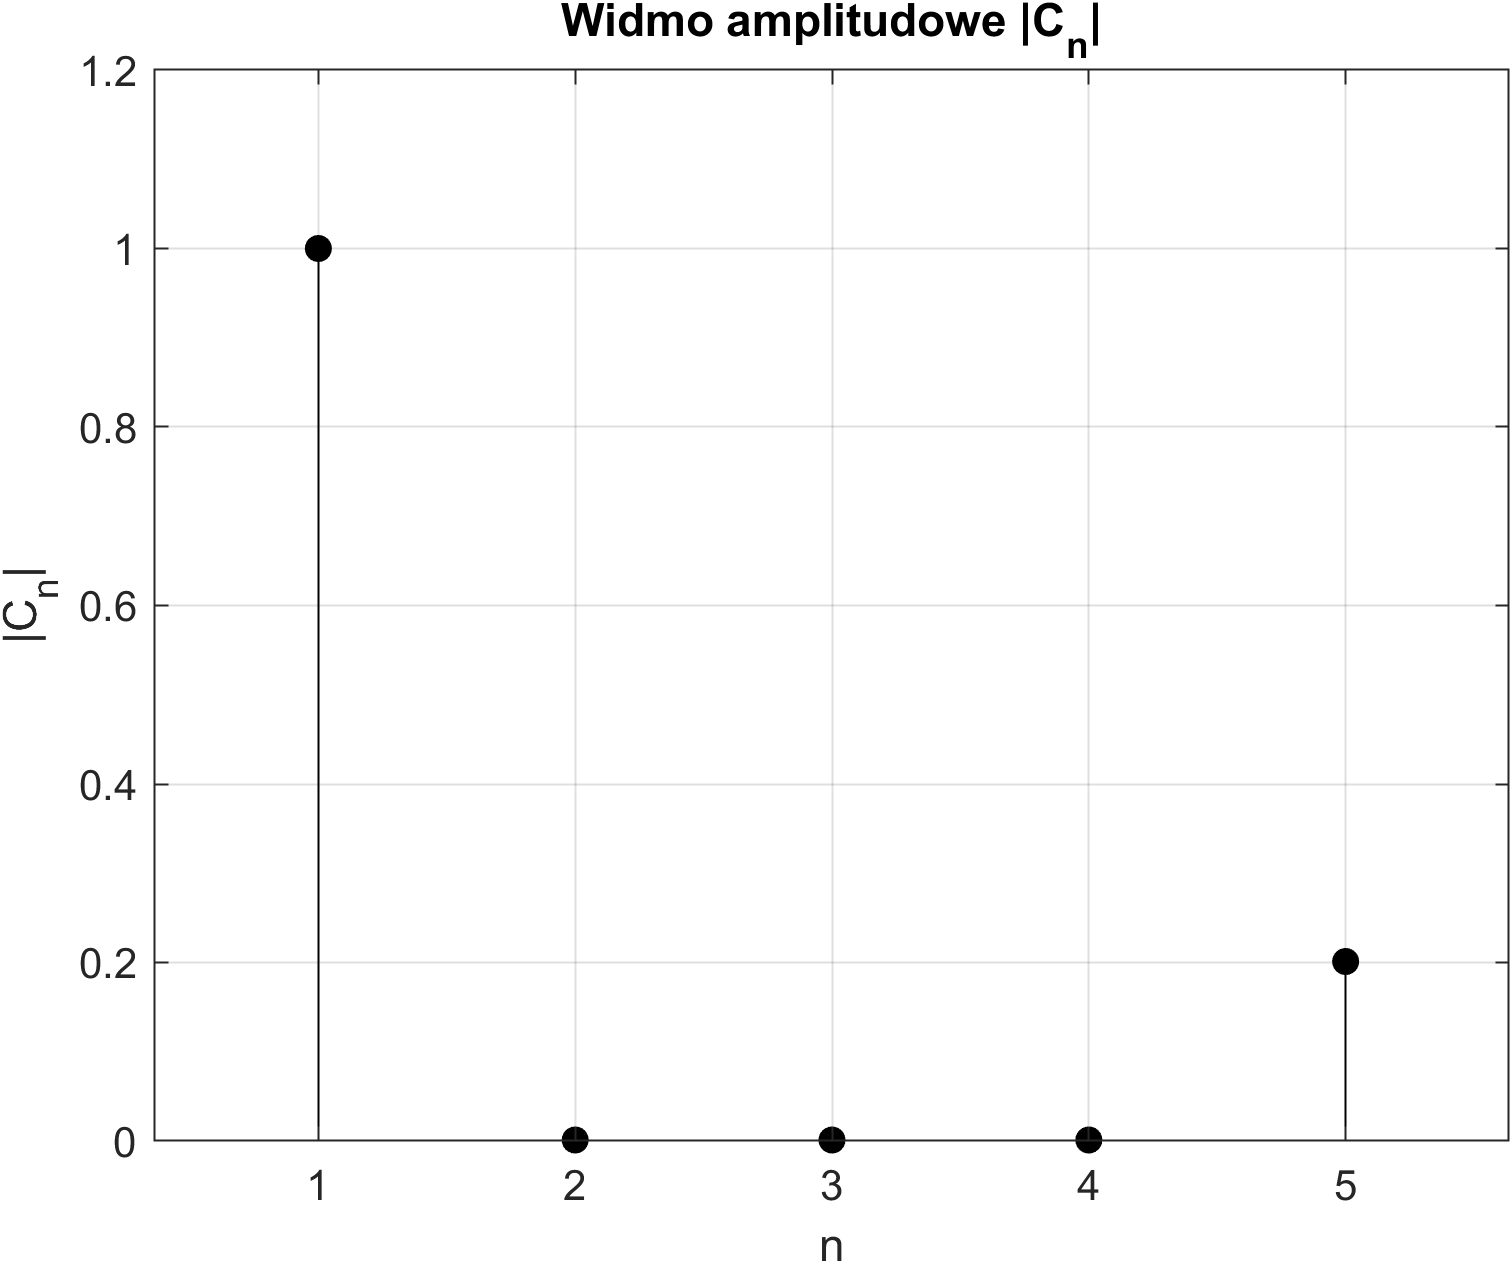
\includegraphics[width=\linewidth]{src/Lab005/spectrum.png}
		\label{fig:lab5_spectrum}
	\end{subfigure}
	\caption{Obrazy wyniku działania algorytmu rozkładu w szereg.}
\end{figure}

\subsection{Zadanie 2}

\subsubsection{Treść}

Wykorzystując dwuwymiarową transformatę Fouriera zaproponuj jego implementację oraz wykonaj
eksperymenty z filtracją środkowo przepustową obrazu tęczówki oka podanej przez prowadzącego.
Poniżej przedstawiono przykładowe rezultaty uzyskane dla obrazu Lena z wykorzystaniem maski
prostokątnej.

\subsubsection{Przykładowy program}

\lstinputlisting[style= matlabStyle, caption= Algorytm rozkładu w szereg Fouriera, label=Lab005_l2]{src/Lab005/zadanie2.m}

\subsubsection{Obrazy}

\begin{figure}[H]
	\centering
	\begin{subfigure}[t]{0.45\linewidth}
		\centering
		
\includegraphics[width=\linewidth]{src/lab005/zad2_iris_original.png}
		\label{fig:lab5z2_original}
	\end{subfigure}
	
	\centering
	\begin{subfigure}[t]{0.45\linewidth}
		\centering
		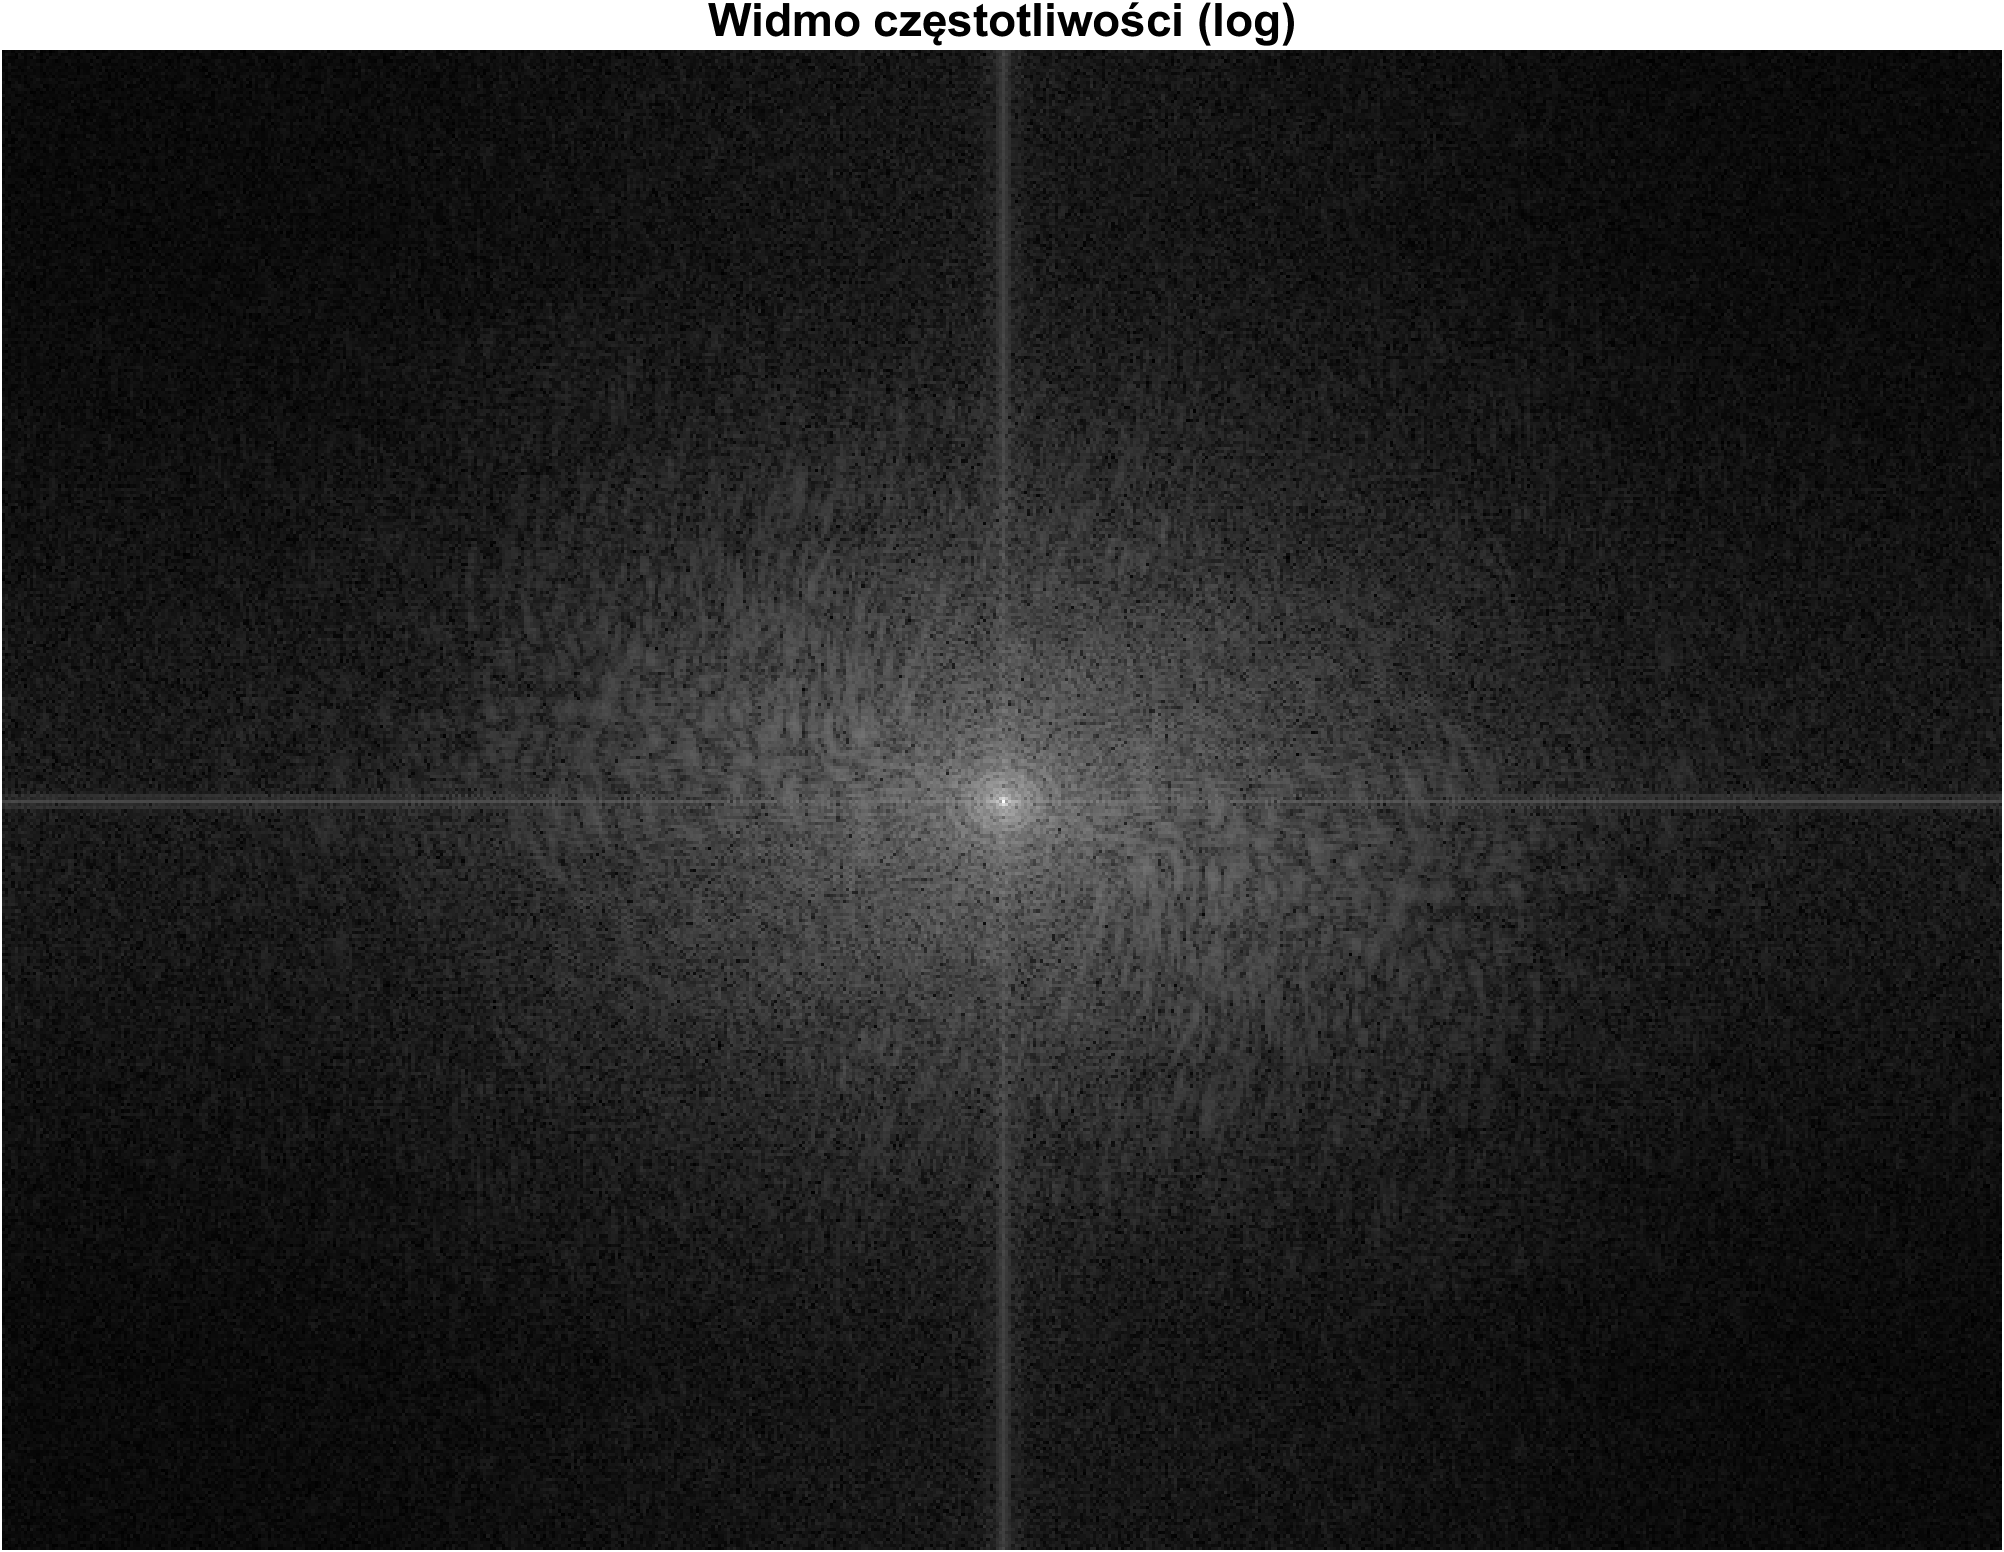
\includegraphics[width=\linewidth]{src/Lab005/zad2_iris_fft_spectrum.png}
		\label{fig:lab5z2_spectrum}
	\end{subfigure}
	\hfill
	\begin{subfigure}[t]{0.45\linewidth}
		\centering
		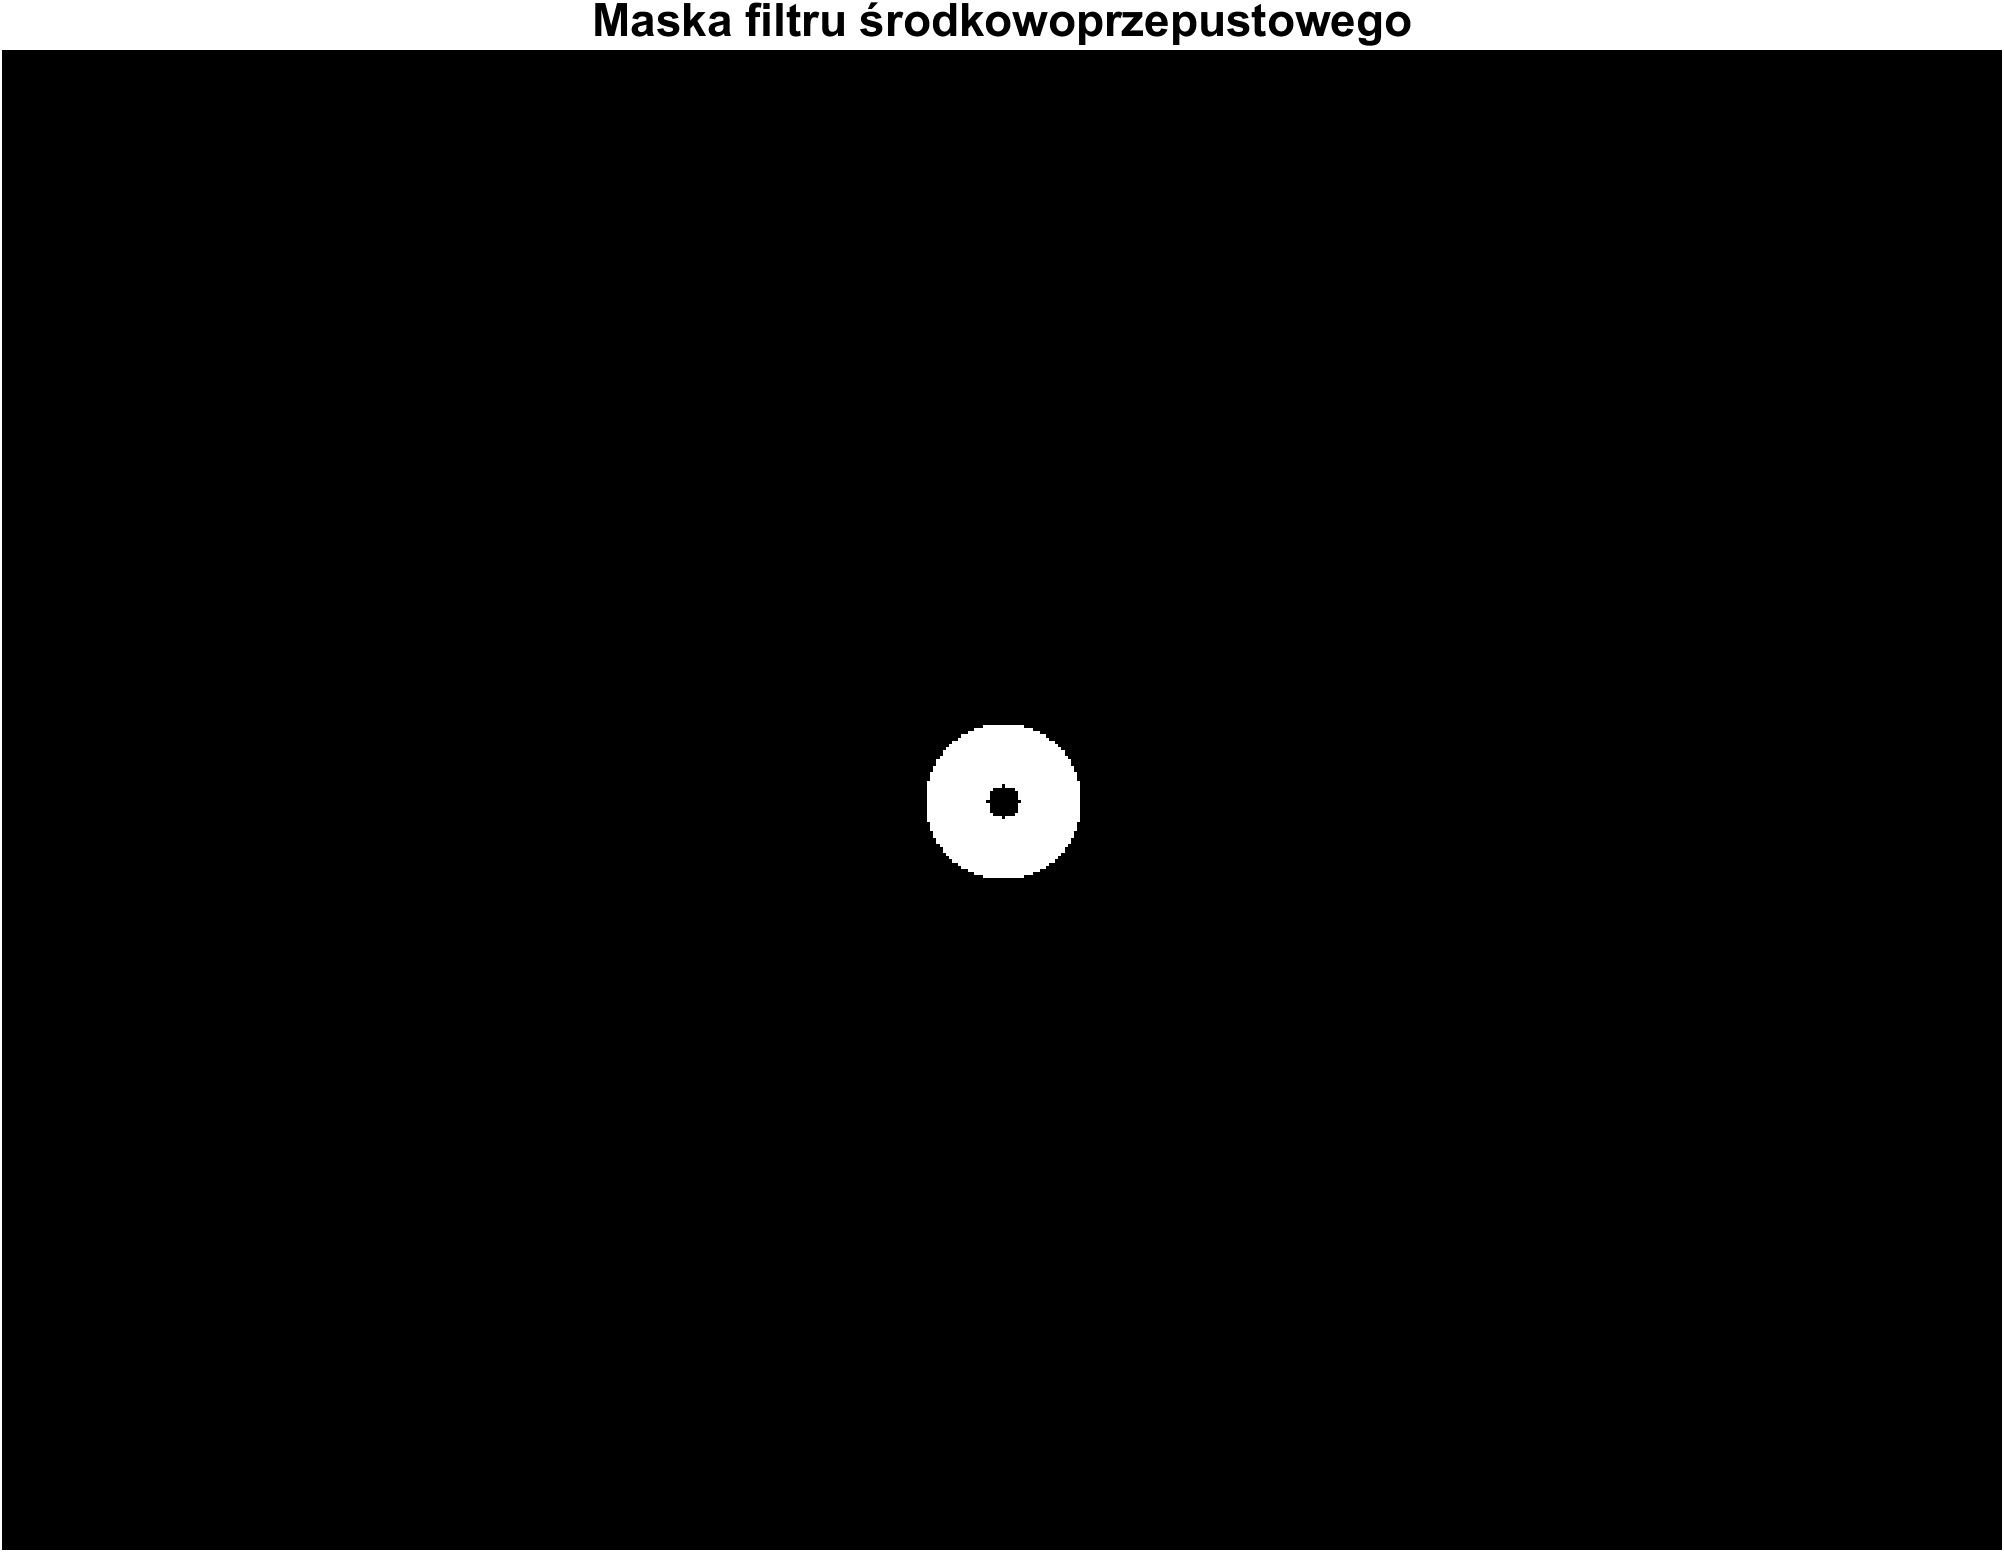
\includegraphics[width=\linewidth]{src/Lab005/zad2_iris_filter_mask.png}
		\label{fig:lab5z2_mask}
	\end{subfigure}
	
	\centering
	\begin{subfigure}[t]{0.45\linewidth}
		\centering
		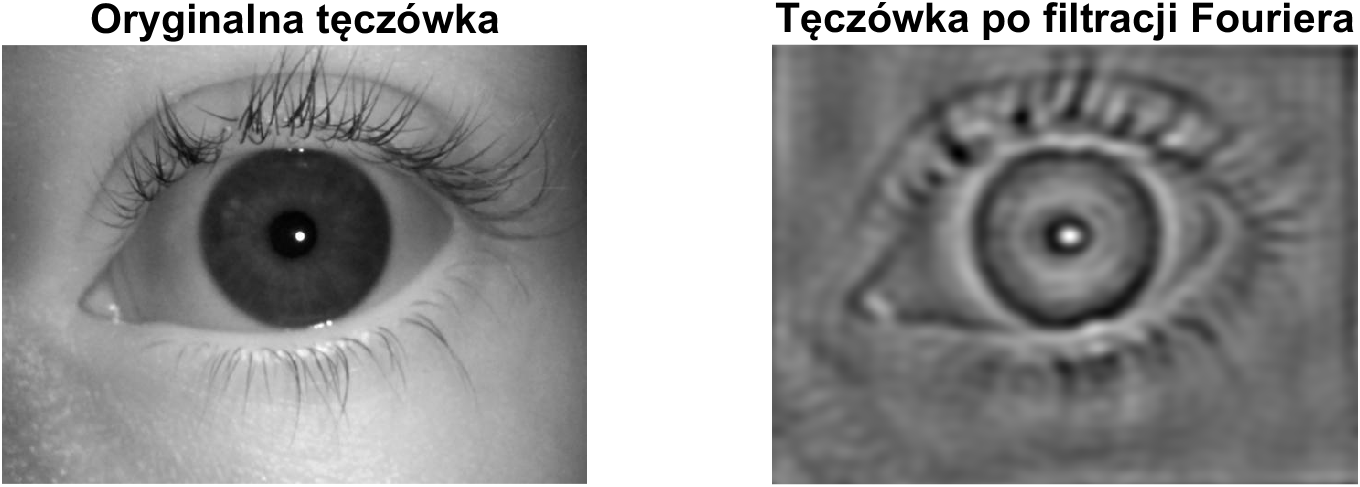
\includegraphics[width=\linewidth]{src/Lab005/zad2_iris_comparison.png}
		\label{fig:lab5z2_comparison}
	\end{subfigure}
	\hfill
	\begin{subfigure}[t]{0.45\linewidth}
		\centering
		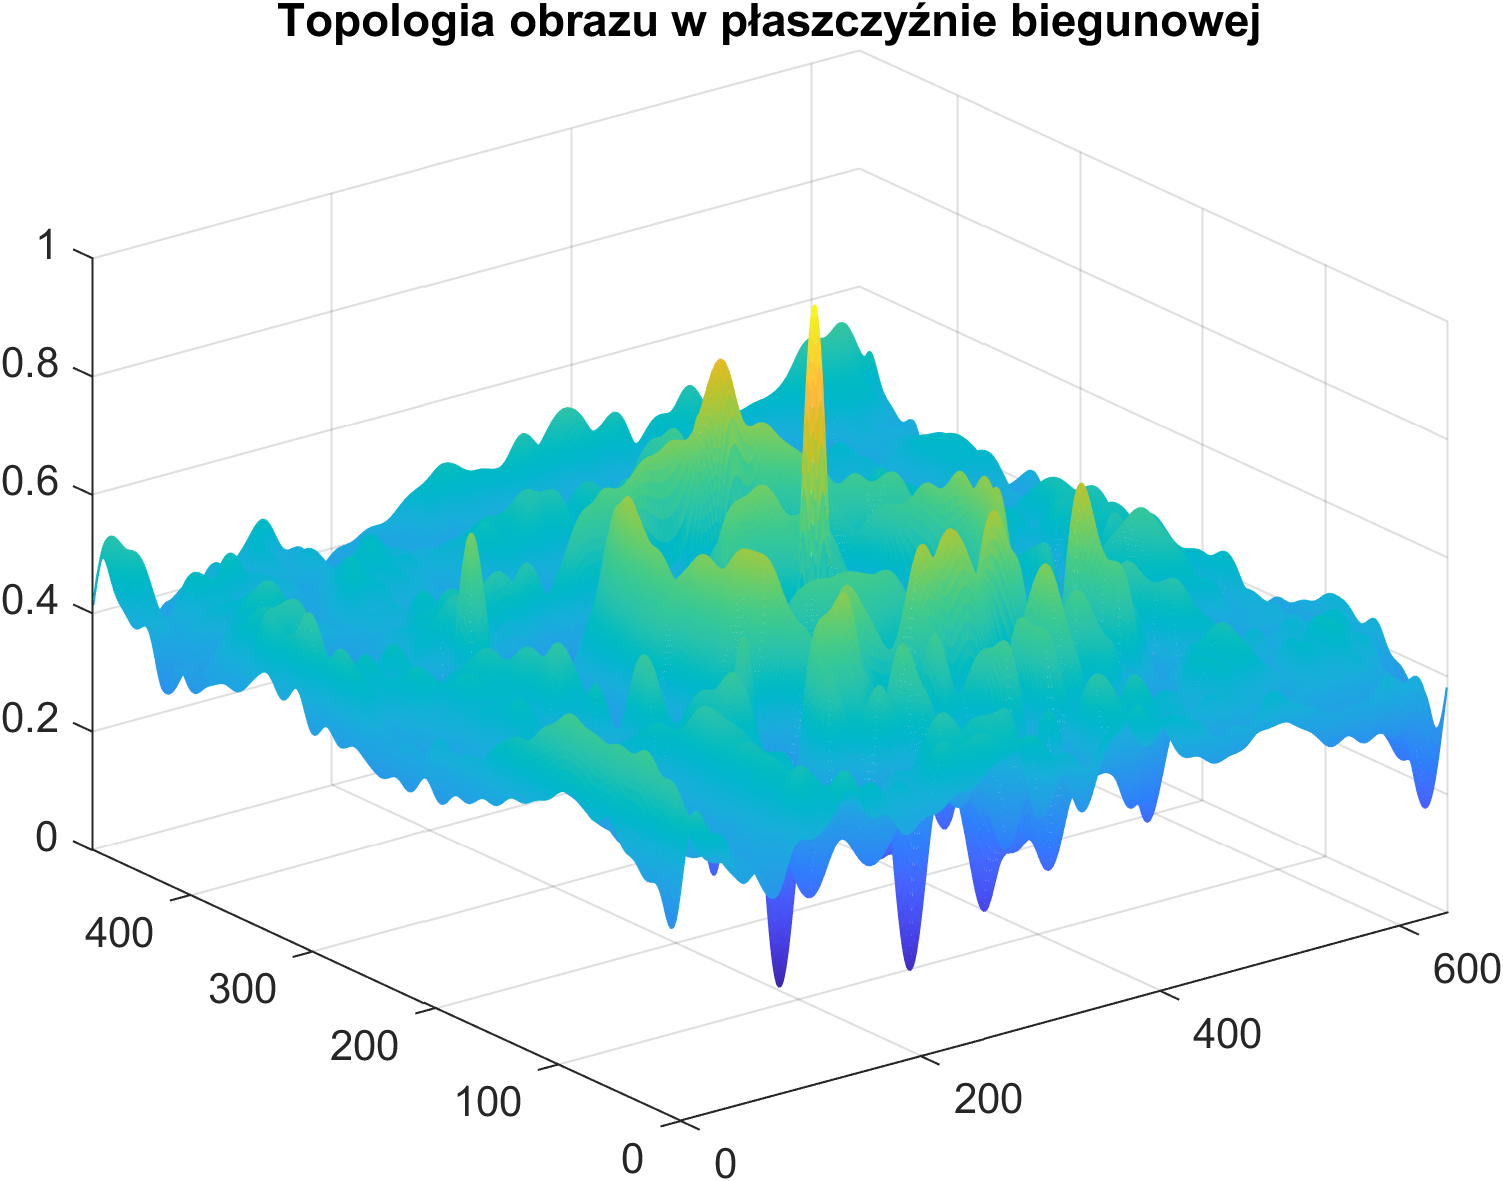
\includegraphics[width=\linewidth]{src/Lab005/zad2_iris_surface_plot.png}
		\label{fig:lab5_surface}
	\end{subfigure}
\end{figure}

\subsection{Zadanie 3}

\subsubsection{Treść}

Przetestuj przedstawiony powyżej mechanizm filtracji częstotliwościowej na obrazie
daktyloskopijnym.

\subsubsection{Przykładowy program}

\lstinputlisting[style= matlabStyle, caption= Algorytm rozkładu w szereg Fouriera, label=Lab005_l3]{src/Lab005/zadanie3.m}

\subsubsection{Obrazy}

\begin{figure}[H]
	\centering
	\begin{subfigure}[t]{0.45\linewidth}
		\centering
		
\includegraphics[width=\linewidth]{src/lab005/fingerprint_original.png}
		\label{fig:lab5z3_original}
	\end{subfigure}
	\hfill
	\begin{subfigure}[t]{0.45\linewidth}
		\centering
		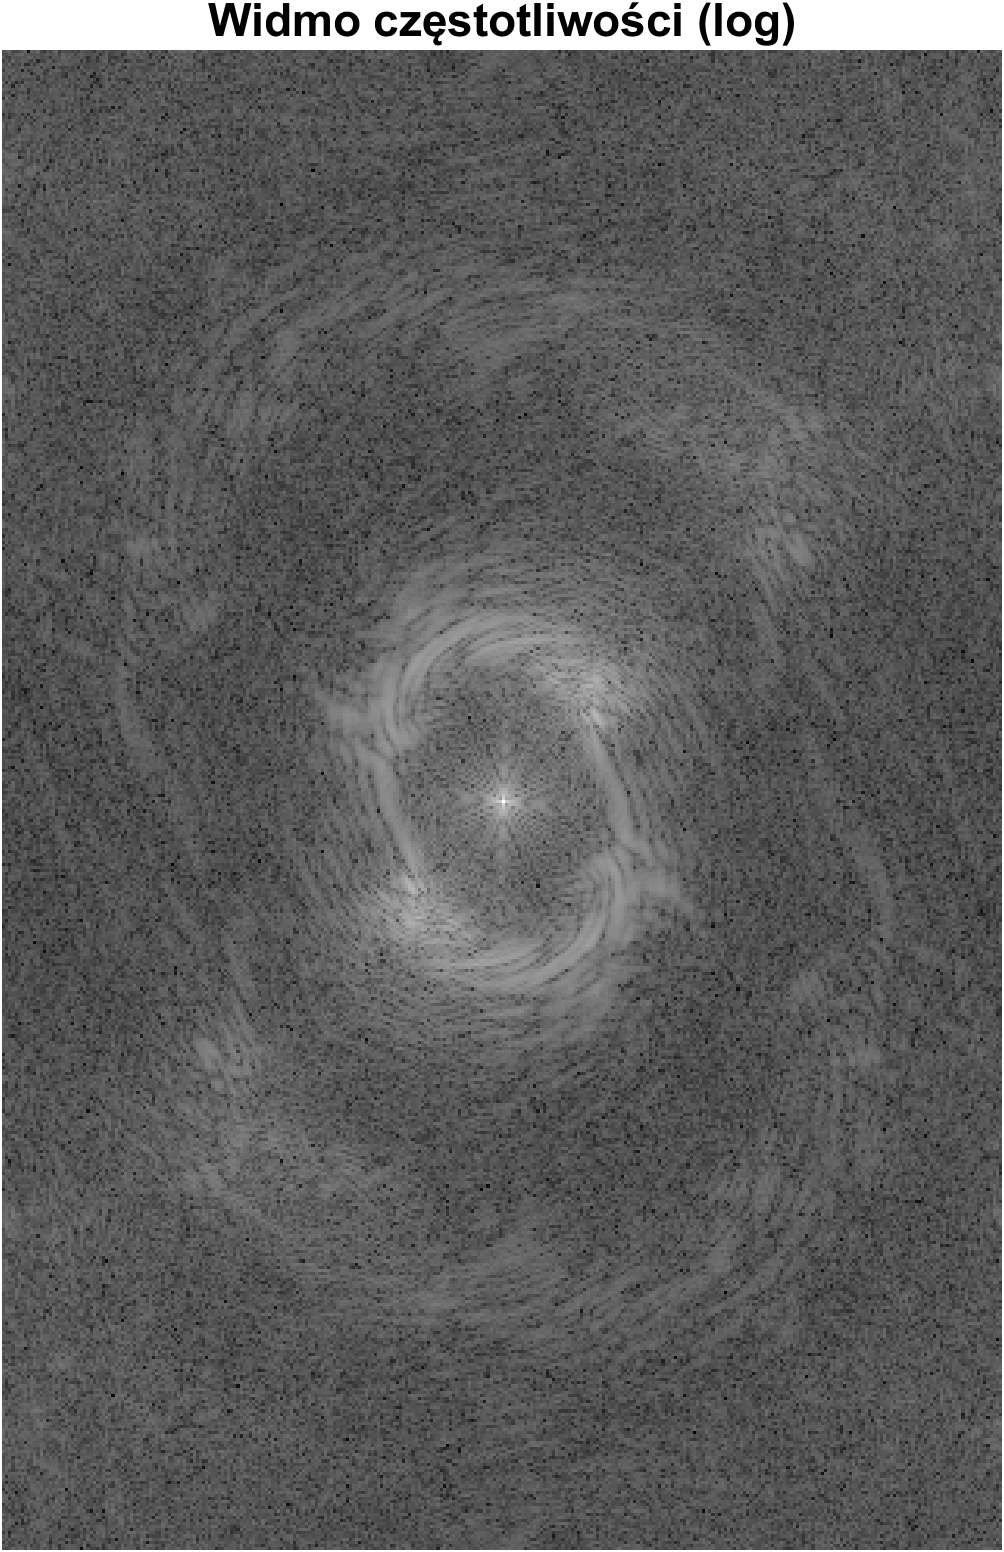
\includegraphics[width=\linewidth]{src/Lab005/fingerprint_fft_spectrum.png}
		\label{fig:lab5z3_spectrum}
	\end{subfigure}
	
	\centering
	\begin{subfigure}[t]{0.45\linewidth}
		\centering
		
\includegraphics[width=\linewidth]{src/Lab005/fingerprint_filter_mask.png}
		\label{fig:labz3_mask}
	\end{subfigure}
	\hfill
	\begin{subfigure}[t]{0.45\linewidth}
		\centering
		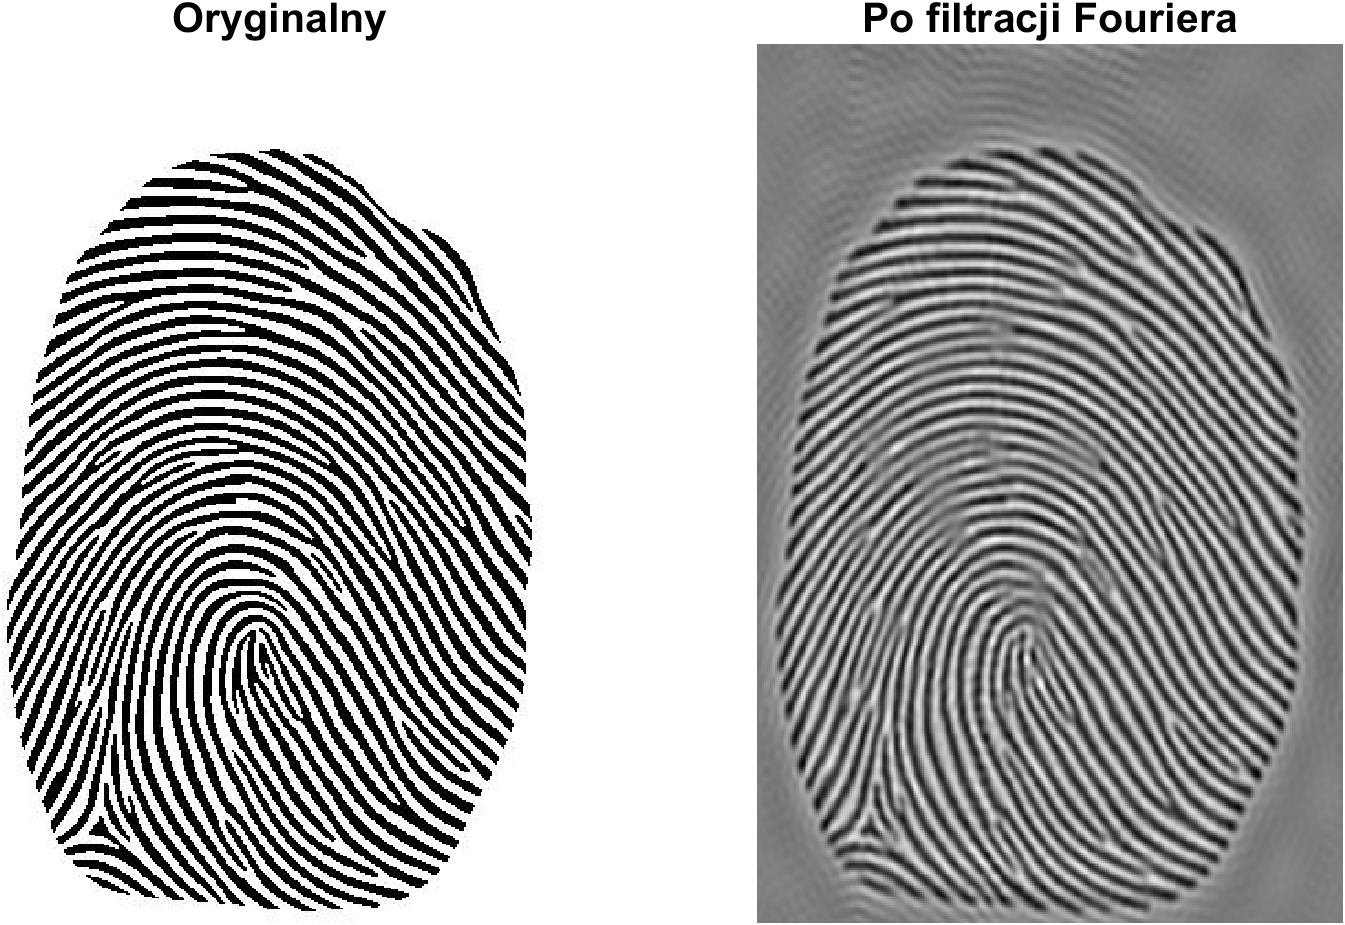
\includegraphics[width=\linewidth]{src/Lab005/fingerprint_comparison.png}
		\label{fig:lab5z3_comparison}
	\end{subfigure}
\end{figure}

\section{Wnioski}

Na podstawie przeprowadzonych eksperymentów można stwierdzić, że:

\subsection{Zadanie 1 – Szereg Fouriera dla sygnału okresowego}
\begin{itemize}
	\item Szereg Fouriera umożliwia rozkład złożonego sygnału okresowego na sumę składowych harmonicznych (sinusoidalnych).
	\item Liczba uwzględnionych harmonicznych (\texttt{roz}) znacząco wpływa na jakość rekonstrukcji – większa liczba pozwala dokładniej odwzorować kształt sygnału.
	\item Współczynniki $A_n$ i $B_n$ opisują odpowiednio składowe kosinusowe i sinusowe sygnału. Ich analiza pozwala zrozumieć udział poszczególnych częstotliwości.
	\item Rekonstrukcja sygnału z ograniczonej liczby harmonicznych jest skuteczna, lecz może prowadzić do efektu Gibbsa na nieciągłościach.
\end{itemize}

\subsection{Zadanie 2 – Filtracja obrazu tęczówki (2D FFT)}
\begin{itemize}
	\item Dwuwymiarowa transformata Fouriera pozwala analizować zawartość częstotliwościową obrazu i stosować filtry bezpośrednio w dziedzinie częstotliwości.
	\item Filtr środkowoprzepustowy skutecznie eliminuje zarówno niskie częstotliwości (np. niejednolite oświetlenie), jak i wysokie (szumy), pozostawiając najistotniejsze struktury tęczówki.
	\item Poprawiona zostaje czytelność wzorca tęczówki, co jest przydatne w systemach biometrycznych.
	\item Prosta maska w postaci pierścienia (idealny filtr pasmowy) jest łatwa do implementacji i daje dobre efekty wizualne.
\end{itemize}

\subsection{Zadanie 3 – Filtracja obrazu daktyloskopijnego (odcisk palca)}
\begin{itemize}
	\item Obraz odcisku palca również można skutecznie analizować i przetwarzać w dziedzinie częstotliwości przy użyciu 2D FFT.
	\item Filtracja środkowoprzepustowa umożliwia eliminację tła i szumów, wzmacniając jednocześnie struktury grzbietów i bruzd.
	\item Wynikowy obraz po filtracji zawiera bardziej wyraziste cechy, co ułatwia dalsze etapy przetwarzania, takie jak wykrywanie minutiae.
	\item Odpowiedni dobór zakresu częstotliwości w masce filtru ma kluczowe znaczenie dla jakości uzyskanego obrazu.
\end{itemize}



\chapter{Laboratorium 6}
\label{cha:Lab006}
\makeatletter


% *********************************************************************
% w poniższej metryczce należy uzupełnić informacje o:
% - temacie ćwiczenia
% - numer ćwiczenia
% - numer grupy laboratoryjnej
% - numer zespołu
% - datę wykonania ćwiczenia oraz oddania ćwiczenia.
% *********************************************************************

\begin{table}[H]
    \centering
    \renewcommand{\tabularxcolumn}[1]{m{#1}}  % Dostosowanie kolumny do zawartości
    \newcolumntype{C}{>{\centering\arraybackslash}X}
    \begin{tabularx}{\linewidth}{|C|C|}
        \hline
        \multicolumn{2}{|c|}{\makecell{\textbf{\Large{Biometryczne Systemy Zabezpieczeń}} \\ \textbf{Ćwiczenia Laboratoryjne}}} \\ \hline
        \multicolumn{1}{|l|}{Temat}                    &              OBRAZY DAKTYLOSKOPIJNE TOKENIZACJA- METODA PROSTA I GRAFOWA , TOKENIZACJA TĘCZÓWKI OKA ALGORYTM JOHNA DAUGMANA            \\ \hline
        \multicolumn{1}{|l|}{Ćwiczenie nr:}                    &      06                   \\ \hline
        \multicolumn{1}{|l|}{Autorzy:}                         &   \@author                              \\ \hline
        \multicolumn{1}{|l|}{Grupa laboratoryjna}                       &       02               \\ \hline
        \multicolumn{1}{|l|}{Zespół nr. }                       &    XX                  \\ \hline
        \multicolumn{1}{|l|}{Data wykonana ćwiczenia}         &  06.05.2025     \\ \hline
        \multicolumn{1}{|l|}{Data oddania ćwiczenia  }         &   13.05.2025     \\ \hline
    \end{tabularx}
\end{table}


\section{Cel ćwiczenia}

Celem laboratorium jest zrozumienie procesu tokenizacji w kontekście danych biometrycznych oraz
praktyczna implementacja algorytmów do ekstrakcji cech z obrazów daktyloskopijnych (minucje) oraz
porównanie prostych i grafowych metod dopasowania tokenów. Zastosowanie algorytmu Johna
Daugmana do tokenizacji pola tęczówki oka oraz wyznaczanie miary podobieństwa poprzez obliczenie
dystansu Hamminga.

\section{Wstęp teoretyczny}

Obrazy daktyloskopijne (ang. \textit{fingerprint images}) to obrazy przedstawiające wzór linii papilarnych palca, składający się z charakterystycznych grzbietów (\textit{ridge}) i dolin (\textit{valley}). Te lokalnie periodyczne struktury są unikalne dla każdej osoby i stanowią podstawę systemów biometrycznych opartych na rozpoznawaniu odcisków palców.

Etapy przetwarzania obrazu daktyloskopijnego można zestawić w następującej kolejności:

\begin{enumerate}
	\item \textbf{Pozyskiwanie obrazu (Image Acquisition)} – rejestracja obrazu odcisku palca przy użyciu skanera optycznego, pojemnościowego, ultradźwiękowego itp.
	\item \textbf{Wstępne przetwarzanie (Preprocessing)} – korekcja kontrastu, usuwanie szumu, poprawa jakości obrazu.
	\item \textbf{Wzmocnienie i filtrowanie (Enhancement \& Filtering)} – zastosowanie filtrów (np. Gabora) w celu uwydatnienia struktury linii papilarnych.
	\item \textbf{Binaryzacja i ścienianie (Binarization \& Thinning)} – przekształcenie obrazu do formy binarnej (0/1) i redukcja grubości linii do 1 piksela.
	\item \textbf{Ekstrakcja minucji (Minutiae Extraction)} – wykrywanie punktów charakterystycznych, takich jak zakończenia linii (\textit{ending}) czy rozwidlenia (\textit{bifurcation}).
\end{enumerate}

\subsection*{Model matematyczny obrazu daktyloskopijnego}

Obraz odcisku palca można opisać jako funkcję:
\begin{equation}
	I(x, y): \mathbb{Z}^2 \rightarrow [0,255]
\end{equation}
gdzie $I(x,y)$ oznacza wartość jasności piksela o współrzędnych $(x,y)$. Typowy obraz daktyloskopijny ma rozmiar np. $512 \times 512$ pikseli i rozdzielczość 500~dpi, co odpowiada ok. 19,7~$\mu$m/piksel.

Wzorce linii papilarnych są lokalnie okresowe — grzbiety i doliny mają charakterystyczne częstotliwości przestrzenne. Filtrowanie w dziedzinie częstotliwości pozwala na:
\begin{itemize}
	\item zwiększenie kontrastu grzbietów,
	\item tłumienie szumów,
	\item poprawę jakości detekcji minucji.
\end{itemize}

\subsection*{Filtr Gabora}

Filtr Gabora jest często używanym narzędziem do analizy tekstury w obrazach biometrycznych. Łączy w sobie lokalizację przestrzenną (funkcja Gaussa) i selektywność częstotliwościową (fala sinusoidalna).

Postać filtru Gabora:
\begin{equation}
	G(x, y) = \exp\left( -\frac{x'^2 + \gamma^2 y'^2}{2\sigma^2} \right) \cdot \cos\left(2\pi \frac{x'}{\lambda} + \phi \right)
\end{equation}
gdzie:
\begin{align}
	x' &= x \cos\theta + y \sin\theta \\
	y' &= -x \sin\theta + y \cos\theta
\end{align}

Parametry:
\begin{itemize}
	\item $\lambda$ – długość fali (częstotliwość grzbietu),
	\item $\theta$ – orientacja lokalna grzbietów,
	\item $\phi$ – przesunięcie fazowe (zwykle 0 lub $\pi/2$),
	\item $\sigma$ – skala funkcji Gaussa (rozmycie),
	\item $\gamma$ – eliptyczność filtru.
\end{itemize}

Filtracja obrazu odcisku palca:
\begin{equation}
	I'(x, y) = I(x, y) * G_{\theta(x,y), \lambda(x,y)}(x, y)
\end{equation}

Zastosowanie filtru zwiększa kontrast grzbietów, redukuje szum i poprawia ekstrakcję minucji.

\subsection*{Binaryzacja i szkieletyzacja}

Celem binarnej segmentacji (np. metodą Otsu) jest uzyskanie obrazu 0-1, gdzie linie papilarne są reprezentowane jako ciągi pikseli. Następnie stosuje się \textbf{ścienianie} (ang. \textit{thinning}) w celu sprowadzenia szerokich linii do ich szkieletu o szerokości jednego piksela. Dzięki temu możliwa jest precyzyjna detekcja cech takich jak rozwidlenia i zakończenia linii.

\subsection*{Ekstrakcja i tokenizacja minucji}

Minucje to charakterystyczne punkty na liniach papilarnych:
\begin{itemize}
	\item zakończenia linii (ending),
	\item rozwidlenia (bifurcation).
\end{itemize}

Każda minucja może być opisana trójkątem $(x, y, \theta)$:
\begin{equation}
	M = [x, y, \theta]
\end{equation}

Zestaw takich punktów stanowi token biometryczny. Może on być wykorzystany w systemach dopasowujących, np. poprzez porównanie pozycji i orientacji lub przez analizę struktury grafowej zależności między minucjami.

\subsection*{Usuwanie fałszywych minucji}

Fałszywe minucje mogą powstać w wyniku zakłóceń, obciętych krawędzi obrazu lub niedoskonałości w przetwarzaniu morfologicznym. W celu ich eliminacji stosuje się:
\begin{itemize}
	\item heurystyki geometryczne (odległość, orientacja, pozycja),
	\item ocenę jakości minucji,
	\item metody uczenia maszynowego do klasyfikacji prawdziwych/fałszywych minucji.
\end{itemize}


\section{Opis wykorzystywanego oprogramowania i narzędzi}

\section{Zadania do wykonania samodzielnego}

\subsection{Zadanie 1}

\subsubsection{Treść}

Wykonaj tokenizację wybranej pary obrazów daktyloskopijnych i wyznacz podobieństwa zestawów
wyodrębnionych minucji z wykorzystaniem metody prostej oraz grafowej. Porównaj skuteczność obu
metod.

\subsubsection{Przykładowy program}

\lstinputlisting[style= matlabStyle, caption= Algorytm rozkładu w szereg Fouriera, label=Lab006_l1]{src/Lab006/zadanie1.m}

\subsubsection{Obrazy}

\begin{figure}[H]
	\centering
	\begin{subfigure}[t]{0.45\linewidth}
		\centering
		
\includegraphics[width=\linewidth]{src/lab006/zad1results.png}
		\label{fig:lab6z1_finger1}
	\end{subfigure}
	\hfill
	\begin{subfigure}[t]{0.45\linewidth}
		\centering
		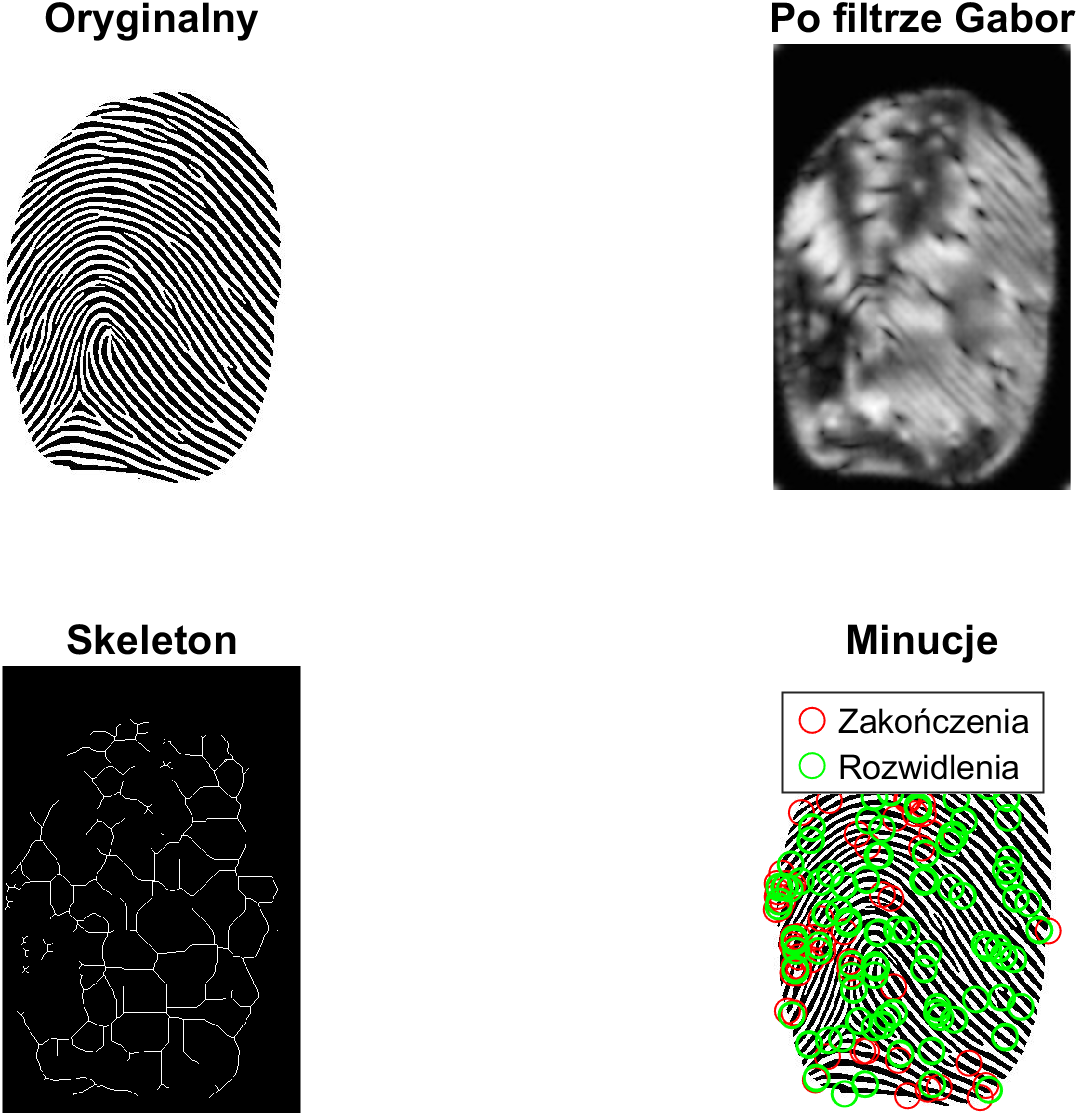
\includegraphics[width=\linewidth]{src/Lab006/zad2results.png}
		\label{fig:lab6z1_finger2}
	\end{subfigure}
\end{figure}

\subsection{Zadanie 2}

\subsubsection{Treść}

Wykonaj tokenizację wybranej podanego zestawu obrazów tęczówki oka i wyznacz dla każdej pary
dystans Hamminga HD. Oceń otrzymane wyniki ze względu na podobieństwo i poziom okluzji pola
tęczówki.

\subsubsection{Przykładowy program}

\lstinputlisting[style= matlabStyle, caption= Algorytm rozkładu w szereg Fouriera, label=Lab006_l2]{src/Lab006/zadanie2.m}

\subsubsection{Obrazy}

% --- Grupa 1: Wyryte tęczówki ---
\begin{figure}[H]
	\centering
	\begin{subfigure}[t]{0.3\linewidth}
		
\includegraphics[width=\linewidth]{src/lab006/output/iris_detected_01.png}
		\caption{Obraz 1}
		\label{fig:lab6z2_iris_detected1}
	\end{subfigure}
	\hfill
	\begin{subfigure}[t]{0.3\linewidth}
		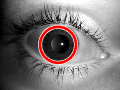
\includegraphics[width=\linewidth]{src/Lab006/output/iris_detected_02.png}
		\caption{Obraz 2}
		\label{fig:lab6z2_iris_detected2}
	\end{subfigure}
	\hfill
	\begin{subfigure}[t]{0.3\linewidth}
		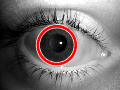
\includegraphics[width=\linewidth]{src/Lab006/output/iris_detected_03.png}
		\caption{Obraz 3}
		\label{fig:lab6z2_iris_detected3}
	\end{subfigure}
	\caption{Wyryte tęczówki}
\end{figure}

% --- Grupa 2: Znormalizowane tęczówki ---
\begin{figure}[H]
	\centering
	\begin{subfigure}[t]{0.3\linewidth}
		
\includegraphics[width=\linewidth]{src/lab006/output/iris_normalized_01.png}
		\caption{Normalizacja 1}
		\label{fig:lab6z2_iris_normalized1}
	\end{subfigure}
	\hfill
	\begin{subfigure}[t]{0.3\linewidth}
		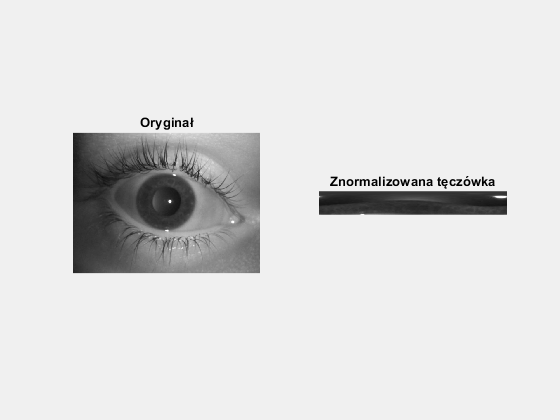
\includegraphics[width=\linewidth]{src/Lab006/output/iris_normalized_02.png}
		\caption{Normalizacja 2}
		\label{fig:lab6z2_iris_normalized2}
	\end{subfigure}
	\hfill
	\begin{subfigure}[t]{0.3\linewidth}
		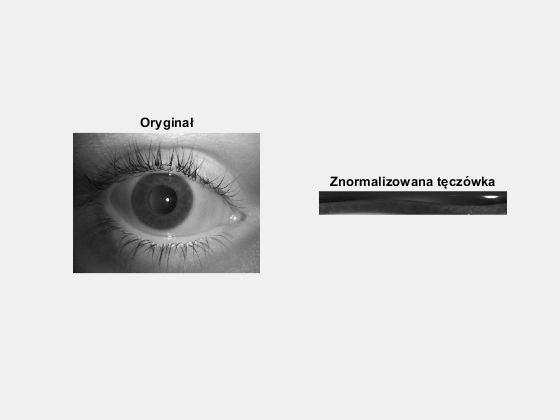
\includegraphics[width=\linewidth]{src/Lab006/output/iris_normalized_03.png}
		\caption{Normalizacja 3}
		\label{fig:lab6z2_iris_normalized3}
	\end{subfigure}
	\caption{Znormalizowane tęczówki}
\end{figure}

% --- Grupa 3: Macierz Hamminga ---
\begin{figure}[H]
	\centering
	
\includegraphics[width=0.5\linewidth]{src/lab006/output/hamming_matrix.png}
	\caption{Macierz dystansu Hamminga}
	\label{fig:lab6z2_matrix}
\end{figure}


\section{Wnioski}

Na podstawie przeprowadzonych eksperymentów można stwierdzić, że:

W normalizacji
\begin{itemize}
	\item Normalizacja obrazu do postaci prostokątnej pozwoliła na wyrównanie różnic wynikających z położenia i wielkości tęczówki w obrazach wejściowych.
	\item Uzyskane postacie normalizowane charakteryzowały się spójną strukturą, co umożliwiło dalsze przetwarzanie.
	\item Segmentacja oparta na założeniu środkowego położenia źrenicy okazała się wystarczająca przy obrazach dobrze wycentrowanych, jednak może nie sprawdzać się w bardziej realistycznych scenariuszach (np. zepsute detekcje, okluzje powiek).
\end{itemize}

W tokenizacji
\begin{itemize}
	\item Tokenizacja z użyciem filtrów Gabora pozwoliła uzyskać binarne wzorce reprezentujące strukturę tęczówki.
	\item Macierz dystansu Hamminga wykazała wyraźne różnice między parami obrazów: najniższe wartości wskazywały na wysokie podobieństwo, natomiast wartości bliskie 0.5 sugerowały brak zgodności (lub silną okluzję).
	\item Okluzje fragmentów tęczówki (np. rzęsy, powieki) znacząco wpływają na zwiększenie dystansu Hamminga, ponieważ maski nie zawsze skutecznie eliminują szumy z tokenów.
	\item Pomimo uproszczeń w modelu, metoda pozwala skutecznie odróżnić obrazy tej samej tęczówki od różnych.
\end{itemize}

Przeprowadzony proces dowodzi, że nawet uproszczona segmentacja i normalizacja umożliwiają wykonanie skutecznej ekstrakcji cech biometrycznych. Dystans Hamminga dobrze sprawdza się jako miara podobieństwa binarnych tokenów i potwierdza, że metoda jest odporna na drobne zakłócenia, choć jej skuteczność zależy od jakości segmentacji i maskowania zakłóceń.

% Wyłączenie działania `ulem` na czas bibliografii
\renewcommand{\emph}[1]{\textit{#1}}
% Bibliografia
% Dodanie bibliografi do spisu treści
\addcontentsline{toc}{section}{\textbf{Bibliografia}}
\bibliographystyle{plain}
\bibliography{bibliografia}

% Przywrócenie działania `ulem`
\renewcommand{\emph}[1]{\uline{#1}}

\clearpage
% Dodanie spisu rysunków do spisu treści
\addcontentsline{toc}{section}{\textbf{Spis rysunków}}
\listoffigures
\clearpage

% Dodanie spisu tabel do spisu treści
\addcontentsline{toc}{section}{\textbf{Spis tabel}}
\listoftables
\clearpage


\clearpage

% Dodanie spisu listingow do spisu treści
\addcontentsline{toc}{section}{\textbf{Spis listingów}}
\lstlistoflistings
\clearpage


% \appendixs
\include{appendix/statement-A}

\end{document}
